%%%%%%%%%%%%%%%%%%%%%%%%%%%%%%%%%%%%%%%%%%%%%%%%%%%%%%%%%%%%%
% Tesis de Pregrado – Universidad del Valle
% Archivo principal reorganizado y optimizado
%%%%%%%%%%%%%%%%%%%%%%%%%%%%%%%%%%%%%%%%%%%%%%%%%%%%%%%%%%%%%

\documentclass[
12pt,
spanish,
singlespacing,
headsepline
]{MastersDoctoralThesis}

%%%%%%%%%%%%%%%%%%%%%%%%%%%%%%%%%%%%%%%%%%%%%%%%%%%%%%%%%%%%%
% PAQUETES BÁSICOS DE IDIOMA, ENCODING, TIPOGRAFÍA
%%%%%%%%%%%%%%%%%%%%%%%%%%%%%%%%%%%%%%%%%%%%%%%%%%%%%%%%%%%%%

\usepackage[utf8]{inputenc}
\usepackage[T1]{fontenc}
\usepackage{babel}
\usepackage{mathpazo} % Fuente Palatino
\usepackage{csquotes} % Requerido por biblatex

%%%%%%%%%%%%%%%%%%%%%%%%%%%%%%%%%%%%%%%%%%%%%%%%%%%%%%%%%%%%%
% PAQUETES MATEMÁTICOS Y ENTORNOS
%%%%%%%%%%%%%%%%%%%%%%%%%%%%%%%%%%%%%%%%%%%%%%%%%%%%%%%%%%%%%

\usepackage{amsmath, amsthm, amsfonts, amssymb, amscd}
\usepackage{braket}        % Notación |ψ⟩
\usepackage{mathrsfs}      % Fuentes caligráficas
\usepackage{enumitem}      % Listas personalizadas
\usepackage{titlesec}      % Control de títulos
\usepackage{microtype}     % Mejora espaciado y evita overfull hbox

%%%%%%%%%%%%%%%%%%%%%%%%%%%%%%%%%%%%%%%%%%%%%%%%%%%%%%%%%%%%%
% PAQUETES GRÁFICOS Y FIGURAS
%%%%%%%%%%%%%%%%%%%%%%%%%%%%%%%%%%%%%%%%%%%%%%%%%%%%%%%%%%%%%

\usepackage{graphicx}
\usepackage{xcolor}

%%%%%%%%%%%%%%%%%%%%%%%%%%%%%%%%%%%%%%%%%%%%%%%%%%%%%%%%%%%%%
% CONFIGURACIÓN DE REFERENCIAS/BIBLIOGRAFÍA
%%%%%%%%%%%%%%%%%%%%%%%%%%%%%%%%%%%%%%%%%%%%%%%%%%%%%%%%%%%%%

\usepackage[
backend=biber,
style=numeric,
natbib=true,
sorting=none
]{biblatex}

\addbibresource{ref.bib}

%%%%%%%%%%%%%%%%%%%%%%%%%%%%%%%%%%%%%%%%%%%%%%%%%%%%%%%%%%%%%
% DEFINICIÓN DE TEOREMAS
%%%%%%%%%%%%%%%%%%%%%%%%%%%%%%%%%%%%%%%%%%%%%%%%%%%%%%%%%%%%%

\theoremstyle{plain}
\newtheorem{theorem}{Teorema}[section]
\newtheorem{lemma}[theorem]{Lema}
\newtheorem{criterion}[theorem]{Criterio}
\newtheorem{proposition}[theorem]{Proposición}
\newtheorem{corollary}[theorem]{Corolario}

\theoremstyle{definition}
\newtheorem{definition}[theorem]{Definición}
\newtheorem{example}[theorem]{Ejemplo}
\newtheorem{exercise}[theorem]{Ejercicio}
\newtheorem{conclusion}[theorem]{Conclusión}
\newtheorem{conjecture}[theorem]{Conjetura}
\newtheorem{axiom}[theorem]{Axioma}
\newtheorem{problem}[theorem]{Problema}

\theoremstyle{remark}
\newtheorem{remark}[theorem]{Observación}

%%%%%%%%%%%%%%%%%%%%%%%%%%%%%%%%%%%%%%%%%%%%%%%%%%%%%%%%%%%%%
% CONFIGURACIÓN DE MÁRGENES (tfg Universidad del Valle)
%%%%%%%%%%%%%%%%%%%%%%%%%%%%%%%%%%%%%%%%%%%%%%%%%%%%%%%%%%%%%

\geometry{
    paper=a4paper,
    inner=2.5cm,
    outer=3.8cm,
    bindingoffset=.5cm,
    top=1.5cm,
    bottom=1.5cm
}

\AddToHook{env/abstract/begin}{\renewcommand{\byname}{por}}

%%%%%%%%%%%%%%%%%%%%%%%%%%%%%%%%%%%%%%%%%%%%%%%%%%%%%%%%%%%%%
% INFORMACIÓN DE TESIS
%%%%%%%%%%%%%%%%%%%%%%%%%%%%%%%%%%%%%%%%%%%%%%%%%%%%%%%%%%%%%

\thesistitle{Retroproyección filtrada en reconstrucción tomográfica: un estudio teórico y computacional}
\supervisor{Julio Delgado}
\author{Kevin Vélez Escarria}
\degree{Pregrado en Matemáticas}
\university{Universidad del Valle}
\department{Departamento de Matemáticas}
\faculty{Facultad de Ciencias Naturales y Exactas}

%%%%%%%%%%%%%%%%%%%%%%%%%%%%%%%%%%%%%%%%%%%%%%%%%%%%%%%%%%%%%
% METADATOS PDF (hipervínculos ya son cargados por la clase)
%%%%%%%%%%%%%%%%%%%%%%%%%%%%%%%%%%%%%%%%%%%%%%%%%%%%%%%%%%%%%
\keywords{ } % espacio en blanco
\AtBeginDocument{
    \hypersetup{
        pdftitle=\ttitle,
        pdfauthor=\authorname,
        pdfkeywords=\keywordnames
    }
}

%%%%%%%%%%%%%%%%%%%%%%%%%%%%%%%%%%%%%%%%%%%%%%%%%%%%%%%%%%%%%
% DOCUMENTO
%%%%%%%%%%%%%%%%%%%%%%%%%%%%%%%%%%%%%%%%%%%%%%%%%%%%%%%%%%%%%

\begin{document}

\frontmatter
\pagestyle{plain}

%%%%%%%%%%%%%%%%%%%%%%%%%%%%%%%%%%%%%%%%%%%%%%%%%%%%%%%%%%%%%
% PORTADA
%%%%%%%%%%%%%%%%%%%%%%%%%%%%%%%%%%%%%%%%%%%%%%%%%%%%%%%%%%%%%

\begin{titlepage}
\begin{center}

\vspace*{0.06\textheight}
{\scshape\LARGE \univname\par}\vspace{1.5cm}
\textsc{\Large Tesis de Pregrado}\\[0.5cm]

\HRule \\[0.4cm]
{\huge \bfseries \ttitle\par}
\HRule \\[1.5cm]

\begin{minipage}[t]{0.4\textwidth}
\begin{flushleft}\large
\textbf{Autor:}\\
Kevin Vélez Escarria
\end{flushleft}
\end{minipage}
\begin{minipage}[t]{0.4\textwidth}
\begin{flushright}\large
\textbf{Director:}\\
Ph.D. Julio Delgado
\end{flushright}
\end{minipage}\\[2.5cm]


\large \textit{Trabajo de grado presentado como requisito para optar por el título de \textbf{Matemático}.} 

\vspace{1cm}
{\large \today}\\[0.3cm]

\includegraphics[scale=0.17]{Figures/logos/logo.pdf}

\end{center}
\end{titlepage}

%%%%%%%%%%%%%%%%%%%%%%%%%%%%%%%%%%%%%%%%%%%%%%%%%%%%%%%%%%%%%
% RESUMEN
%%%%%%%%%%%%%%%%%%%%%%%%%%%%%%%%%%%%%%%%%%%%%%%%%%%%%%%%%%%%%

\begin{abstract}
\addchaptertocentry{\abstractname}
Esta tesis estudia el problema de reconstruir una imagen a partir de sus proyecciones, una situación central en la tomografía computarizada. El punto de partida es la transformada de Radon, que modela matemáticamente la información obtenida al medir integrales de una imagen sobre rectas. A partir de este modelo se analiza la retroproyección filtrada, un método clásico que permite aproximar la imagen original mediante una combinación de herramientas de Fourier y retroproyección.

El trabajo combina una presentación teórica del método con una implementación computacional reproducible. En la parte matemática se introducen las convenciones usadas para la transformada de Radon, la retroproyección y la fórmula de inversión por retroproyección filtrada. En la parte numérica se construye un fantoma geométrico, se generan sus proyecciones y se comparan reconstrucciones obtenidas con el filtro rampa y con varias modificaciones de este filtro.

Los experimentos permiten observar el papel del filtro en la calidad de la reconstrucción. En ausencia de ruido, los filtros más cercanos a la rampa conservan mejor los detalles de la imagen; en presencia de ruido, los filtros que atenúan ciertas frecuencias pueden producir reconstrucciones más estables, aunque con pérdida de resolución. Así, la tesis muestra que la retroproyección filtrada no depende solo de una fórmula de inversión, sino también del equilibrio entre detalle, estabilidad y sensibilidad al ruido introducido por la elección del filtro.
\end{abstract}

%%%%%%%%%%%%%%%%%%%%%%%%%%%%%%%%%%%%%%%%%%%%%%%%%%%%%%%%%%%%%
% CONTENIDO PRINCIPAL
%%%%%%%%%%%%%%%%%%%%%%%%%%%%%%%%%%%%%%%%%%%%%%%%%%%%%%%%%%%%%

\mainmatter
\pagestyle{thesis}

\tableofcontents

\chapter*{Introducción}
\addchaptertocentry{Introducción}
\markboth{Introducción}{Introducción}

La tomografía computarizada (TC) es una técnica de diagnóstico por imágenes que permite reconstruir cortes transversales de un objeto a partir de mediciones externas de rayos X. Su desarrollo combina física, tecnología y matemática: las mediciones no entregan directamente la imagen interna, sino información indirecta obtenida a lo largo de trayectorias de rayos, lo que ubica la reconstrucción tomográfica dentro del marco de los problemas inversos \cite{kirsch2011}. En un modelo bidimensional idealizado, una sección del objeto se representa mediante una función que describe el coeficiente de atenuación, y los datos medidos se interpretan como integrales de esa función sobre rectas. Esta descripción conduce naturalmente a la transformada de Radon, introducida originalmente por Johann Radon en 1917 \cite{radon1917}.

Desde el punto de vista físico, el vínculo entre mediciones e integrales de línea proviene de la ley de Beer--Lambert. En un modelo ideal de rayos paralelos, al normalizar la intensidad medida y tomar logaritmos se obtiene una cantidad igual a la integral del coeficiente de atenuación sobre la trayectoria recorrida por el haz. Al repetir este proceso para distintas posiciones del detector y distintos ángulos de adquisición, los datos se organizan en un sinograma. Esta formulación constituye el punto de partida matemático de la reconstrucción tomográfica \cite{barrett_swindell1996,kuchment2014}.

El problema central consiste en reconstruir la función desconocida a partir de su transformada de Radon. En el modelo continuo, el teorema de corte de Fourier relaciona la transformada de Fourier de las proyecciones con valores de la transformada de Fourier bidimensional de la imagen. Esta relación permite derivar una fórmula de inversión mediante un cambio a coordenadas polares en frecuencia. El factor de densidad que aparece en ese cambio de variables da lugar al filtro rampa, cuyo símbolo es $|\sigma|$ bajo la convención de Fourier adoptada en esta tesis.

La retroproyección filtrada, o FBP por sus siglas en inglés, implementa esta idea en dos pasos: primero filtra cada proyección en la variable del detector mediante un multiplicador de Fourier y luego retroproyecta las proyecciones filtradas sobre el dominio espacial. La rampa clásica será la referencia teórica y computacional del método. Sin embargo, su crecimiento en altas frecuencias también explica la sensibilidad del procedimiento frente al ruido \cite[Cap.~3]{kak_slaney1988}\cite[Sec.~V.1]{natterer2001}; por ello, en la parte computacional se estudia una familia etiquetada A--F, explorada previamente en una contribución presentada en MAPI~4 \cite{velez_lopez2026mapi4}. Las definiciones matemáticas exactas empleadas en esta tesis se presentan en el Capítulo~3.

El diseño y análisis de filtros para FBP continúa siendo un tema activo, tanto desde el punto de vista de estimaciones de error como de la optimización de funciones filtro \cite{beckmann_iske2017,beckmann_nickel2025}. En esta tesis, los filtros A--F se usan con un propósito exploratorio y no reproducen los filtros optimizados de esos trabajos.

El objetivo de esta tesis es estudiar la retroproyección filtrada en reconstrucción tomográfica bidimensional desde una perspectiva teórica y computacional. En la parte teórica se fijan las convenciones de Fourier, se define la transformada de Radon, se deriva la retroproyección como adjunto formal y se obtiene la fórmula de FBP. En la parte computacional se analizan simulaciones reproducibles con un fantoma geométrico propio, sinogramas discretos y ruido controlado.

El alcance se limita a la geometría paralela bidimensional, al fantoma geométrico principal, al filtro rampa como referencia y a una familia A--F de filtros para comparación. No se pretende modelar un sistema clínico tridimensional ni establecer un filtro universalmente óptimo.

La estructura del trabajo es la siguiente. En el primer capítulo se presentan los preliminares estrictamente necesarios: convenciones de Fourier, nociones mínimas de operadores lineales y adjuntos, y multiplicadores de Fourier. En el segundo capítulo se desarrolla el modelo tomográfico continuo, la transformada de Radon, la retroproyección, el teorema de corte de Fourier y la fórmula de retroproyección filtrada. El tercer capítulo se dedica a la discretización, la implementación numérica y la comparación espectral y visual de filtros en reconstrucciones simuladas. El trabajo termina con conclusiones y líneas futuras.

\chapter{Preliminares}

\label{Preliminares}

\section{Espacios de Hilbert y espacios de funciones}
\label{Spaces}

En esta sección se fija el marco funcional en el que se formularán los problemas inversos asociados a la tomografía computarizada. En particular, se introducen los espacios de Hilbert, los espacios $L^{p}$ y los espacios de Sobolev que se utilizarán en los capítulos posteriores. Las referencias generales son \cite{rynne_youngson2000,kirsch2011,natterer2001,kuchment2014}.


\subsection{Espacios de Hilbert}

A lo largo de este trabajo se consideran espacios vectoriales sobre $\mathbb{R}$, a menos que se indique lo contrario.

\begin{definition}
Sea $H$ un espacio vectorial real. Un \emph{producto interno} en $H$ es una aplicación
\[
\langle \cdot,\cdot \rangle : H \times H \to \mathbb{R}
\]
tal que, para todo $x,y,z \in H$ y todo $\alpha \in \mathbb{R}$, se verifican:
\begin{enumerate}
  \item $\langle \alpha x + y, z \rangle = \alpha \langle x,z \rangle + \langle y,z \rangle$;
  \item $\langle x,y \rangle = \langle y,x \rangle$ ;
  \item $\langle x,x \rangle \ge 0$;
  \item $\langle x,x \rangle = 0$ implica $x=0$ .
\end{enumerate}
En este caso se dice que $(H,\langle \cdot,\cdot \rangle)$ es un \emph{espacio con producto interno}.
\end{definition}


\begin{proposition}

    Sea $H$ un espacio con producto interno, y sean $x, y \in X$, entonces
    \begin{itemize}
        \item $|\langle x,y \rangle|^2 \leq \langle x, y \rangle \langle y, y \rangle $
        \item La función $|| \cdot || : X \to \mathbb{R}$ definida por $|| x || = \langle x, x \rangle ^{1/2}$ es una norma en $X$.
    \end{itemize}
\end{proposition}

\begin{proof}
    Pendiente
\end{proof}

\begin{definition}
Un espacio con producto interno $(H,\langle \cdot,\cdot \rangle)$ se denomina \emph{espacio de Hilbert} si es completo con respecto a la norma inducida $\|\cdot\|$, es decir, si toda sucesión de Cauchy en $(H,\|\cdot\|)$ converge en $H$.
\end{definition}

\begin{example}
Entre los ejemplos básicos de espacios de Hilbert se encuentran:
\begin{enumerate}
  \item El espacio euclídeo $\mathbb{R}^{n}$ con el producto interno
  \[
  \langle x,y \rangle = \sum_{j=1}^{n} x_{j} y_{j}.
  \]
  \item El espacio
  \[
  \ell^{2} = \Bigl\{ (x_{j})_{j \in \mathbb{N}} : \sum_{j=1}^{\infty} |x_{j}|^{2} < \infty \Bigr\},
  \]
  con producto interno
  \[
  \langle x,y \rangle = \sum_{j=1}^{\infty} x_{j} y_{j}.
  \]
  \item El espacio $L^{2}(\Omega)$, donde $\Omega \subset \mathbb{R}^{n}$ es un conjunto medible, con
  \[
  \langle f,g \rangle = \int_{\Omega} f(x)\,g(x)\,dx.
  \]
\end{enumerate}
\end{example}

En el contexto de la tomografía computarizada, los espacios de Hilbert de funciones, en particular los espacios $L^{2}(\Omega)$ y ciertos espacios de Sobolev, proporcionan un marco natural para la formulación de los problemas directo e inverso asociados a la transformada de Radon \cite{natterer2001,kuchment2014}.


\subsection{Espacios \texorpdfstring{$L^{p}$}{Lp}}

Sea $(X,\mathcal{A},\mu)$ un espacio de medida. Para $1 \le p < \infty$, se define
\[
L^{p}(X) = \left\{ f: f \text{ es medible y }  \int_{X} |f(x)|^{p}\, d\mu(x) < \infty \right\},
\]
La aplicación
\[
\|f\|_{L^{p}} := \left( \int_{X} |f(x)|^{p}\, d\mu(x) \right)^{1/p}
\]
define una norma en $L^{p}(X)$, y con esta norma $L^{p}(X)$ es un espacio de Banach \cite{rynne_youngson2000}.

Para $p = \infty$, primero definimos el supremo esencial.

\begin{definition}[Supremo esencial]
Sea $f : X \to \mathbb{R}$ una función medible. Se define el \emph{supremo esencial}
de $|f|$ como
\[
\operatorname*{ess\,sup}_{x\in X} |f(x)|
:= \inf\Bigl\{ M \ge 0 : \mu\bigl(\{x \in X : |f(x)| > M\}\bigr) = 0 \Bigr\}.
\]
\end{definition}

\begin{definition}[Espacio $L^{\infty}$]
Se define
\[
L^{\infty}(X) 
= \Bigl\{ f \text{ medible} : \operatorname*{ess\,sup}_{x\in X} |f(x)| < \infty \Bigr\},
\]
identificando funciones que coinciden casi en todas partes. La aplicación
\[
\|f\|_{L^{\infty}} := \operatorname*{ess\,sup}_{x\in X} |f(x)|
\]
define una norma en $L^{\infty}(X)$, con la cual $L^{\infty}(X)$ es un espacio de Banach.
\end{definition}

El caso $p=2$ será especialmente relevante en lo que sigue. En este caso, $L^{2}(X)$ es un espacio de Hilbert con el producto interno
\[
\langle f,g \rangle_{L^{2}} = \int_{X} f(x)\,g(x)\, d\mu(x).
\]
En particular, espacios del tipo $L^{2}(\mathbb{R}^{2})$ y $L^{2}(\Omega)$, con $\Omega \subset \mathbb{R}^{2}$, se utilizarán para modelar las imágenes y los datos de proyección en los problemas tomográficos \cite{natterer2001,kuchment2014}.


\subsection{Espacios de Sobolev}

Los espacios de Sobolev permiten cuantificar la regularidad de funciones en términos de derivadas (en sentido débil) controladas en norma $L^{2}$. Esta estructura es adecuada para formular hipótesis de suavidad sobre la solución de un problema inverso y para introducir términos de regularización.

Sea $\Omega \subset \mathbb{R}^{n}$ un abierto. Se denota por $C_{c}^{\infty}(\Omega)$ el conjunto de funciones suaves con soporte compacto contenido en $\Omega$.

\begin{definition}[Espacio $L^{1}_{\mathrm{loc}}(\Omega)$]
Se define el espacio de funciones localmente integrables como
\[
L^{1}_{\mathrm{loc}}(\Omega)
= \left\{ f : \Omega \to \mathbb{R} \text{ medible} \;\middle|\;
f \in L^{1}(K) \text{ para todo compacto } K \subset \Omega \right\}.
\]
\end{definition}


\begin{definition}[Derivada débil de primer orden]
Sea $f \in L^{1}_{\mathrm{loc}}(\Omega)$ y $1 \le j \le n$. Se dice que una función $g \in L^{1}_{\mathrm{loc}}(\Omega)$ es la \emph{derivada débil} de $f$ respecto a $x_{j}$ si
\[
\int_{\Omega} f(x)\, \frac{\partial \varphi}{\partial x_{j}}(x)\, dx
= - \int_{\Omega} g(x)\, \varphi(x)\, dx
\quad \text{para toda } \varphi \in C_{c}^{\infty}(\Omega).
\]
En este caso se escribe $g = \partial_{x_{j}} f$.
\end{definition}

\begin{definition}[Espacio de Sobolev $H^{1}(\Omega)$]
Se define
\[
H^{1}(\Omega) = \left\{ f \in L^{2}(\Omega) : \partial_{x_{j}} f \in L^{2}(\Omega) \text{ para todo } j=1,\dots,n \right\},
\]
donde las derivadas se entienden en el sentido débil. La norma en $H^{1}(\Omega)$ viene dada por
\[
\|f\|_{H^{1}(\Omega)}^{2} 
= \int_{\Omega} |f(x)|^{2}\,dx 
+ \sum_{j=1}^{n} \int_{\Omega} \left|\partial_{x_{j}} f(x)\right|^{2}\,dx.
\]
\end{definition}

\begin{proposition}
El espacio $H^{1}(\Omega)$, provisto del producto interno
\[
\langle f,g \rangle_{H^{1}(\Omega)}
= \int_{\Omega} f(x)\,g(x)\,dx
+ \sum_{j=1}^{n} \int_{\Omega} \partial_{x_{j}} f(x)\,\partial_{x_{j}} g(x)\,dx,
\]
es un espacio de Hilbert.
\end{proposition}

\begin{proof}
Pendiente
\end{proof}

Para órdenes superiores resulta conveniente utilizar la notación de multiíndices. Si $\alpha = (\alpha_{1},\dots,\alpha_{n}) \in \mathbb{N}_{0}^{n}$ y $|\alpha| = \alpha_{1} + \cdots + \alpha_{n}$, se escribe
\[
D^{\alpha} f = \partial_{x_{1}}^{\alpha_{1}} \cdots \partial_{x_{n}}^{\alpha_{n}} f,
\]
entendiendo las derivadas en sentido débil.

\begin{definition}[Espacios de Sobolev $H^{k}(\Omega)$]
Sea $k \in \mathbb{N}$. Se define
\[
H^{k}(\Omega) = \left\{ f \in L^{2}(\Omega) : D^{\alpha} f \in L^{2}(\Omega) \text{ para todo multiíndice } \alpha \text{ con } |\alpha|\le k \right\},
\]
con norma
\[
\|f\|_{H^{k}(\Omega)}^{2}
= \sum_{|\alpha|\le k} \int_{\Omega} |D^{\alpha} f(x)|^{2}\,dx.
\]
\end{definition}

Con esta norma, $H^{k}(\Omega)$ es también un espacio de Hilbert \cite{kirsch2011}. En aplicaciones a tomografía, estos espacios permiten formular términos de regularización que penalizan la falta de suavidad de la imagen a reconstruir, típicamente mediante funcionales de la forma
\[
\|Rf - g\|_{Y}^{2} + \alpha \|f\|_{H^{1}(\Omega)}^{2},
\]
donde $R$ denota la transformada de Radon, $g$ representa los datos medidos, $Y$ es un espacio de Hilbert adecuado para el sinograma y $\alpha>0$ es un parámetro de regularización. Estos aspectos se retomarán en capítulos posteriores.



\section{Operadores lineales y operadores compactos}
\label{Operators}

En esta sección se introducen las nociones de operador lineal acotado entre espacios normados y, en particular, entre espacios de Hilbert, así como el concepto de operador adjunto y de operador compacto. Estas herramientas serán fundamentales para la formulación abstracta de los problemas inversos considerados más adelante, donde la transformada de Radon y sus operadores asociados se describen como operadores lineales entre espacios de Hilbert \cite{kirsch2011,natterer2001,kuchment2014}.


\subsection{Operadores lineales acotados}

Sea $X$ un espacio normado sobre $\mathbb{R}$ con norma $\|\cdot\|_{X}$ y sea $Y$ otro espacio normado con norma $\|\cdot\|_{Y}$.

\begin{definition}
Una aplicación $T : X \to Y$ se denomina \emph{operador lineal} si satisface
\[
T(x + y) = T(x) + T(y), \qquad T(\alpha x) = \alpha\,T(x)
\]
para todo $x,y \in X$ y todo $\alpha \in \mathbb{R}$.
\end{definition}

En el contexto de espacios normados, el concepto de acotación equivale al de continuidad en sentido global.

\begin{definition}
Un operador lineal $T : X \to Y$ se dice \emph{acotado} si existe una constante $C \ge 0$ tal que
\[
\|T x\|_{Y} \le C\,\|x\|_{X} \quad \text{para todo } x \in X.
\]
El menor $C$ que verifica la desigualdad anterior se denomina \emph{norma de operador} de $T$ y se denota por
\[
\|T\| := \sup_{\|x\|_{X} = 1} \|T x\|_{Y}.
\]
\end{definition}

Es bien conocido que un operador lineal $T : X \to Y$ es acotado si y solo si es continuo (en cualquier punto de $X$), y que el conjunto de todos los operadores lineales acotados de $X$ en $Y$, denotado por $\mathcal{L}(X,Y)$, es un espacio de Banach con la norma de operador cuando $Y$ es completo \cite{rynne_youngson2000}.

En el caso particular de espacios de Hilbert, se utilizará de forma sistemática la notación $\mathcal{L}(H_{1},H_{2})$ para designar el espacio de todos los operadores lineales acotados de un espacio de Hilbert $H_{1}$ en otro espacio de Hilbert $H_{2}$. Cuando $H_{1} = H_{2} = H$, se escribe simplemente $\mathcal{L}(H)$.


\subsection{Operadores acotados en espacios de Hilbert y operador adjunto}

Sea en adelante $H_{1}$ y $H_{2}$ espacios de Hilbert reales, con productos internos $\langle \cdot,\cdot \rangle_{H_{1}}$ y $\langle \cdot,\cdot \rangle_{H_{2}}$, respectivamente.

Dado un operador lineal acotado $T \in \mathcal{L}(H_{1},H_{2})$ y un vector fijo $y \in H_{2}$, la aplicación
\[
H_{1} \ni x \longmapsto \langle T x, y \rangle_{H_{2}}
\]
es un funcional lineal y acotado sobre $H_{1}$. El teorema de representación de Riesz garantiza que todo funcional lineal continuo sobre un espacio de Hilbert puede representarse mediante un producto interno con un elemento del propio espacio.

\begin{theorem}[Representación de Riesz]
Sea $H$ un espacio de Hilbert real y sea $F : H \to \mathbb{R}$ un funcional lineal y continuo. Entonces existe un único elemento $z \in H$ tal que
\[
F(x) = \langle x,z \rangle_{H} \quad \text{para todo } x \in H.
\]
Además, se cumple $\|F\| = \|z\|_{H}$.
\end{theorem}

\begin{proof}
    Pendiente, tomar de \cite{rynne_youngson2000}
\end{proof}

\begin{definition}[Operador adjunto]
Sea $T \in \mathcal{L}(H_{1},H_{2})$. El \emph{adjunto} de $T$ es el operador $T^{*} \in \mathcal{L}(H_{2},H_{1})$ caracterizado por la propiedad
\[
\langle T x, y \rangle_{H_{2}} = \langle x, T^{*} y \rangle_{H_{1}}
\quad \text{para todo } x \in H_{1}, \; y \in H_{2}.
\]
\end{definition}

\begin{proposition}
Para todo $T \in \mathcal{L}(H_{1},H_{2})$ existe un único operador adjunto $T^{*} \in \mathcal{L}(H_{2},H_{1})$. Además, se cumple
\[
\|T^{*}\| = \|T\|.
\]
\end{proposition}

\begin{proof}
Pendiente
\end{proof}

En el caso $H_{1} = H_{2} = H$, un operador $T \in \mathcal{L}(H)$ se denomina:

\begin{itemize}
  \item \emph{autoadjunto} si $T^{*} = T$;
  \item \emph{positivo} si $T$ es autoadjunto y $\langle T x,x \rangle_{H} \ge 0$ para todo $x \in H$.
\end{itemize}

Este tipo de operadores aparecerá de forma natural al considerar operadores de la forma $T^{*}T$ en problemas inversos lineales.


\subsection{Operadores compactos}

Para describir ciertas características de los problemas mal puestos, resulta conveniente introducir el concepto de operador compacto. Intuitivamente, un operador compacto transforma conjuntos acotados en conjuntos relativamente compactos.

\begin{definition}
Sea $X$ e $Y$ espacios normados. Un operador lineal acotado $K : X \to Y$ se dice \emph{compacto} si para todo conjunto acotado $B \subset X$, la imagen $K(B)$ tiene cierre compacto en $Y$.
\end{definition}

En espacios de Banach (y en particular en espacios de Hilbert), esta definición es equivalente a una caracterización secuencial.

\begin{proposition}
Sea $K \in \mathcal{L}(X,Y)$, donde $X$ e $Y$ son espacios normados. El operador $K$ es compacto si y solo si para toda sucesión acotada $(x_{n}) \subset X$ la sucesión $(Kx_{n})$ posee una subsucesión convergente en $Y$.
\end{proposition}

\begin{proof}
    Pendiente, buscar en \cite{rynne_youngson2000}
\end{proof}


\begin{example}
Ejemplos típicos de operadores compactos entre espacios de Hilbert son:
\begin{enumerate}
  \item Operadores de rango finito: si $T : H_{1} \to H_{2}$ es lineal y $\dim(\operatorname{ran} T) < \infty$, entonces $T$ es compacto.
  \item Ciertos operadores integrales: si $\Omega \subset \mathbb{R}^{n}$ es acotado y $k \in L^{2}(\Omega \times \Omega)$, el operador
  \[
  K f(x) = \int_{\Omega} k(x,y)\,f(y)\,dy
  \]
  define un operador compacto de $L^{2}(\Omega)$ en $L^{2}(\Omega)$ bajo hipótesis adicionales sobre el núcleo $k$ (véase \cite{kirsch2011,natterer2001}).
\end{enumerate}
\end{example}

En espacios de Hilbert, los operadores compactos autoadjuntos admiten una descripción espectral particularmente simple.

\begin{theorem}[Espectro de operadores compactos autoadjuntos]
Sea $H$ un espacio de Hilbert y sea $K \in \mathcal{L}(H)$ un operador compacto y autoadjunto. Entonces existen una sucesión (finita o numerable) de valores propios reales $(\lambda_{j})$ con $\lambda_{j} \to 0$ y un sistema ortonormal de vectores propios $(e_{j}) \subset H$ tal que
\[
K x = \sum_{j} \lambda_{j} \,\langle x,e_{j} \rangle_{H}\, e_{j},
\]
donde la serie converge en $H$ para todo $x \in H$. Además, el espectro de $K$ está formado por $\{0\}$ y, a lo sumo, una sucesión numerable de valores propios reales de multiplicidad finita que solo pueden acumularse en $0$.
\end{theorem}

\begin{proof}
    Pendiente
\end{proof}

Este resultado es una versión del teorema espectral para operadores compactos autoadjuntos; una demostración detallada puede consultarse en \cite{kirsch2011}. En el estudio de problemas inversos lineales, las propiedades espectrales de operadores compactos son fundamentales para entender la aparición de inestabilidades: la presencia de valores propios (o valores singulares) que tienden a cero está directamente relacionada con la falta de estabilidad de la inversión.

En capítulos posteriores se revisará cómo ciertos operadores asociados a la transformada de Radon pueden modelarse, en espacios adecuados, como operadores lineales acotados que presentan características similares a las de los operadores compactos, y cómo esta estructura se refleja en la formulación y análisis de métodos de regularización.

\section{Problemas inversos lineales y regularización}

En esta sección se introduce la formulación abstracta de los problemas inversos lineales en espacios de Hilbert y se presenta el planteamiento clásico de Hadamard sobre problemas bien y mal planteados. Finalmente, se describe de manera preliminar el esquema de regularización de Tikhonov, que se utilizará posteriormente en el estudio del problema inverso asociado a la transformada de Radon. Las referencias principales son \cite{kirsch2011,natterer2001,kuchment2014}.


\subsection{Formulación de Hadamard}

Sea $X$ un espacio de Hilbert que modela el espacio de parámetros o incógnitas, y sea $Y$ otro espacio de Hilbert que modela el espacio de datos. Un problema directo lineal se puede formular abstractamente como
\[
K x = y, \quad x \in X, \; y \in Y,
\]
donde $K \in \mathcal{L}(X,Y)$ es un operador lineal acotado conocido. Dado $x \in X$, el valor $y = Kx$ representa los datos que se observan. El problema inverso correspondiente consiste en determinar $x$ a partir de una observación (aproximada) de $y$.

La noción clásica de problema bien planteado se debe a Hadamard.

\begin{definition}[Hadamard]
Sea $F : X \to Y$ una aplicación. Se dice que el problema
\[
F(x) = y
\]
está \emph{bien planteado} (o es \emph{bien condicionado}) en el sentido de Hadamard si se verifican las siguientes condiciones:
\begin{enumerate}
  \item \textbf{Existencia:} Para todo $y$ en un conjunto de datos de interés, existe al menos un $x \in X$ tal que $F(x) = y$.
  \item \textbf{Unicidad:} Para todo $y$ en dicho conjunto, existe a lo sumo un $x \in X$ que satisfaga $F(x) = y$.
  \item \textbf{Dependencia continua de los datos:} La solución depende continuamente de los datos; más precisamente, si $(y_{n})$ es una sucesión en $Y$ con $y_{n} \to y$ y $x_{n}$ es la solución correspondiente a $y_{n}$, entonces $x_{n} \to x$ en $X$.
\end{enumerate}
Si alguna de estas condiciones falla, se dice que el problema está \emph{mal planteado} (o es \emph{mal condicionado}).
\end{definition}

En el caso lineal, cuando $F = K \in \mathcal{L}(X,Y)$, la existencia y la unicidad están relacionadas con las propiedades algebraicas de $K$ (núcleo y rango), mientras que la dependencia continua se vincula con la continuidad del operador inverso. Esta última es precisamente la fuente de las inestabilidades características de muchos problemas inversos.


\subsection{Problemas inversos lineales en espacios de Hilbert}

En lo que sigue, se considera un operador lineal acotado $K \in \mathcal{L}(X,Y)$ entre espacios de Hilbert reales $X$ e $Y$. El problema directo consiste en calcular $y = Kx$ a partir de $x \in X$. El problema inverso asociado consiste en recuperar $x$ a partir de $y$.

Desde un punto de vista abstracto, el problema inverso lineal puede interpretarse como el problema de invertir el operador $K$. Si $K$ es biyectivo, el teorema de la función inversa implica que $K^{-1} : Y \to X$ es también lineal y acotado, de modo que el problema está bien planteado en el sentido de Hadamard \cite{rynne_youngson2000}. Sin embargo, en la mayoría de las aplicaciones de tomografía, el operador que modela el problema inverso no es biyectivo sobre todo $Y$, o su inverso no es continuo en el rango de $K$.

Incluso cuando $K$ es inyectivo, suele ocurrir que el rango $\operatorname{ran} K$ no es cerrado en $Y$. En tal caso, el operador inverso
\[
K^{-1} : \operatorname{ran} K \to X,
\]
definido por $K^{-1}(y) = x$ cuando $Kx = y$, no es acotado. De manera equivalente, pequeñas perturbaciones de los datos en $\operatorname{ran} K$ pueden producir grandes variaciones en la solución. Esta falta de estabilidad es una característica típica de los problemas inversos lineales mal planteados \cite{kirsch2011}.

El siguiente resultado proporciona un criterio útil en el caso inyectivo.

\begin{proposition}
Sea $K \in \mathcal{L}(X,Y)$ un operador lineal acotado e inyectivo entre espacios de Hilbert. Entonces el operador inverso
\[
K^{-1} : \operatorname{ran} K \to X
\]
es continuo si y solo si el subespacio $\operatorname{ran} K$ es cerrado en $Y$.
\end{proposition}

\begin{proof}
Pendiente \cite{kirsch2011}
\end{proof}

En particular, si $K$ es inyectivo y compacto entre espacios de Hilbert infinitodimensionales, se tiene que $\operatorname{ran} K$ no puede ser cerrado salvo en el caso trivial; por tanto, el problema inverso asociado es mal planteado en el sentido de Hadamard. Esta situación es típica de muchos problemas inversos modelados por operadores integrales, donde la compacidad refleja un efecto de suavizado en las soluciones \cite{kirsch2011,natterer2001}.

En tomografía computarizada, el operador asociado a la transformada de Radon (en espacios adecuados de funciones) presenta un comportamiento análogo al de ciertos operadores compactos o ``cuasi compactos'', en el sentido de que su inversión amplifica inevitablemente el ruido de alta frecuencia presente en los datos. Esta es la razón fundamental por la que, en la práctica, no es posible realizar una inversión ``exacta'' de $K$ a partir de datos ruidosos, y resulta necesario introducir métodos de regularización.


\subsection{Regularización de Tikhonov en el caso lineal}

Una estrategia estándar para tratar problemas inversos lineales mal planteados es sustituir la ecuación $Kx = y$ por un problema variacional bien planteado que compatibilice el ajuste a los datos con un término de penalización que favorezca soluciones ``regulares''. Uno de los métodos más utilizados es la regularización de Tikhonov. La presentación que sigue se basa en \cite{kirsch2011}.

Sea $K \in \mathcal{L}(X,Y)$ un operador lineal acotado entre espacios de Hilbert, y supóngase que los datos disponibles $y^{\delta} \in Y$ satisfacen
\[
\|y^{\delta} - y\|_{Y} \le \delta,
\]
donde $y \in Y$ denota los datos exactos (desconocidos) y $\delta \ge 0$ es un parámetro que representa el nivel de ruido.

Para un parámetro de regularización $\alpha > 0$, se considera el funcional de Tikhonov
\[
J_{\alpha}(x; y^{\delta}) 
= \|Kx - y^{\delta}\|_{Y}^{2} + \alpha \,\|x\|_{X}^{2}, 
\quad x \in X.
\]

\begin{definition}[Solución de Tikhonov]
Sea $\alpha > 0$ y $y^{\delta} \in Y$. Una \emph{solución de Tikhonov} para los datos $y^{\delta}$ con parámetro $\alpha$ es un punto $x_{\alpha}^{\delta} \in X$ que minimiza el funcional $J_{\alpha}(\cdot; y^{\delta})$, es decir,
\[
x_{\alpha}^{\delta} \in \arg\min_{x \in X} J_{\alpha}(x; y^{\delta}).
\]
\end{definition}

El siguiente resultado garantiza la existencia y unicidad de la solución de Tikhonov, así como la ecuación normal que satisface.

\begin{proposition}
Sea $K \in \mathcal{L}(X,Y)$ y $\alpha > 0$. Para todo $y^{\delta} \in Y$ existe un único minimizador $x_{\alpha}^{\delta} \in X$ del funcional $J_{\alpha}(\cdot; y^{\delta})$. Además, $x_{\alpha}^{\delta}$ está caracterizado por la ecuación normal
\[
(K^{*} K + \alpha I) x_{\alpha}^{\delta} = K^{*} y^{\delta},
\]
donde $K^{*} \in \mathcal{L}(Y,X)$ denota el adjunto de $K$ e $I$ es el operador identidad en $X$.
\end{proposition}

\begin{proof}[Idea de la prueba]
El funcional $J_{\alpha}(\cdot; y^{\delta})$ es continuo, estrictamente convexo y coercivo en $X$, debido al término $\alpha \|x\|_{X}^{2}$ con $\alpha>0$. Estas propiedades garantizan la existencia y unicidad del minimizador (véase \cite{kirsch2011}). Para obtener la ecuación normal, se calcula la derivada direccional de $J_{\alpha}$ en la dirección $h \in X$:
\[
\frac{d}{dt} J_{\alpha}(x + t h; y^{\delta})\bigg|_{t=0}
= 2 \langle Kx - y^{\delta}, K h \rangle_{Y} + 2 \alpha \langle x,h \rangle_{X}.
\]
Imponiendo que esta derivada se anula para todo $h \in X$ en el minimizador $x = x_{\alpha}^{\delta}$ y utilizando la definición de operador adjunto, se obtiene
\[
\langle K^{*}(Kx_{\alpha}^{\delta} - y^{\delta}) + \alpha x_{\alpha}^{\delta}, h \rangle_{X} = 0
\quad \text{para todo } h \in X,
\]
lo cual implica
\[
K^{*}(Kx_{\alpha}^{\delta} - y^{\delta}) + \alpha x_{\alpha}^{\delta} = 0,
\]
es decir, $(K^{*}K + \alpha I)x_{\alpha}^{\delta} = K^{*} y^{\delta}$.
\end{proof}

La regularización de Tikhonov define, para cada $\alpha>0$, un operador lineal y acotado $R_{\alpha} : Y \to X$ dado por
\[
R_{\alpha} y^{\delta} = x_{\alpha}^{\delta} = (K^{*}K + \alpha I)^{-1} K^{*} y^{\delta}.
\]
El análisis detallado de las propiedades de $R_{\alpha}$ y del comportamiento de $x_{\alpha}^{\delta}$ cuando $\alpha \to 0$ y $\delta \to 0$ se abordará en un capítulo posterior. De forma muy general, el objetivo es elegir una familia de parámetros $\alpha = \alpha(\delta)$ que permita garantizar la convergencia de $x_{\alpha(\delta)}^{\delta}$ hacia una solución ``generalizada'' del problema inverso $Kx = y$ cuando el nivel de ruido $\delta$ tiende a cero \cite{kirsch2011}.

En el contexto de la tomografía computarizada, la regularización de Tikhonov proporciona un marco natural para estabilizar la reconstrucción de imágenes a partir de sinogramas ruidosos y/o incompletos, ya sea en forma abstracta (como en la ecuación anterior) o incorporando explícitamente términos de suavidad basados en normas de espacios de Sobolev, como las introducidas en la sección anterior.

\chapter{Transformada de Radon y retroproyección filtrada}

En este capítulo se desarrolla el modelo continuo de adquisición tomográfica en geometría paralela y se deriva la fórmula de retroproyección filtrada. Las identidades analíticas se formulan inicialmente para funciones de Schwartz, con las convenciones de Fourier fijadas en el capítulo anterior. El objetivo es obtener, a partir del teorema de corte de Fourier y del cambio a coordenadas polares con radio firmado, la fórmula
\[
f=
\mathcal R^*\mathcal F_t^{-1}
\left[
|\sigma|\,\mathcal F_t(\mathcal Rf)
\right].
\]

\section{Modelo tomográfico y geometría}

En un modelo bidimensional idealizado de tomografía computarizada, una sección del objeto se representa mediante un coeficiente de atenuación
\[
f:\mathbb R^2\to\mathbb R,
\]
no negativo, suficientemente regular y con soporte acotado. Esta función describe la atenuación local que experimenta un haz de rayos X al atravesar el objeto.

La relación física básica entre atenuación y medición se expresa mediante la ley de Beer--Lambert. Si un haz de intensidad inicial $I_0$ recorre una trayectoria $\gamma$ y se mide una intensidad final $I$, entonces, bajo un modelo ideal sin dispersión,
\[
I=I_0\exp\left(-\int_\gamma f(x)\,ds\right).
\]
Por tanto,
\[
-\log\left(\frac{I}{I_0}\right)
=
\int_\gamma f(x)\,ds.
\]
Así, después de normalizar la intensidad y tomar logaritmos, el dato medido es una integral de línea del coeficiente de atenuación. Esta idealización y su conexión con el modelo tomográfico se presentan, por ejemplo, en Kuchment \cite[Sec.~5.3.1, pp.~23--25]{kuchment2014}.

La Figura~\ref{fig:beer-lambert} resume esta etapa física: el detector no mide directamente $f$, sino una intensidad atenuada cuya normalización logarítmica produce una integral sobre la trayectoria del haz.

\begin{figure}[htbp]
\centering
\resizebox{0.86\textwidth}{!}{\shorthandoff{<>}
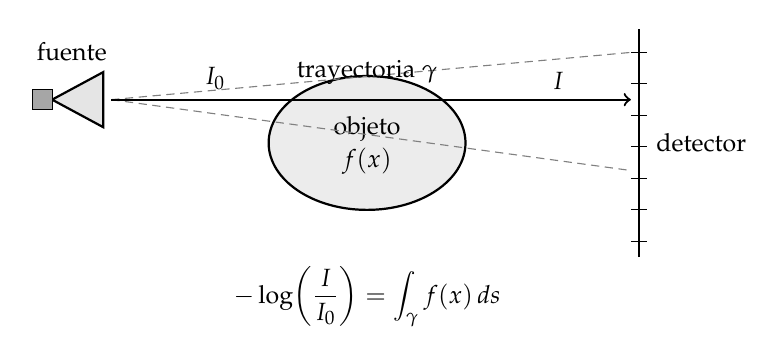
\begin{tikzpicture}[font=\small]
    \draw[draw=black, fill=gray!15, thick] (0,0) ellipse (1.25 and 0.85);
    \node at (0,0.18) {objeto};
    \node at (0,-0.23) {$f(x)$};

    \draw[fill=black!10, draw=black, thick] (-4,0.55) -- (-3.35,0.9) -- (-3.35,0.2) -- cycle;
    \draw[fill=black!35, draw=black] (-4.25,0.42) rectangle (-4,0.68);
    \node[above] at (-3.75,0.92) {fuente};

    \draw[thick] (3.45,-1.45) -- (3.45,1.45);
    \foreach \y in {-1.25,-0.85,...,1.15} {
        \draw[thin] (3.35,\y) -- (3.55,\y);
    }
    \node[right] at (3.55,0) {detector};

    \draw[densely dashed, thin, gray] (-3.25,0.55) -- (3.35,1.15);
    \draw[densely dashed, thin, gray] (-3.25,0.55) -- (3.35,-0.35);
    \draw[->, thick] (-3.25,0.55) -- (3.35,0.55) node[pos=0.20, above] {$I_0$} node[pos=0.86, above] {$I$};
    \node[above] at (0,0.62) {trayectoria $\gamma$};

    \node[align=center, below] at (0,-1.45)
    {$-\log\!\left(\dfrac{I}{I_0}\right)=\displaystyle\int_\gamma f(x)\,ds$};
\end{tikzpicture}
\shorthandon{<>}
}
\caption{Adquisición tomográfica ideal y ley de Beer--Lambert. Elaboración propia.}
\label{fig:beer-lambert}
\end{figure}

En geometría paralela, las trayectorias se modelan por rectas. Para cada $\theta\in[0,\pi)$ se fija
\[
\omega(\theta)=(\cos\theta,\sin\theta),
\qquad
\omega^\perp(\theta)=(-\sin\theta,\cos\theta).
\]
En esta tesis, $\omega(\theta)$ es la normal unitaria a la recta y $\omega^\perp(\theta)$ es la dirección de integración sobre ella. Para $t\in\mathbb R$ se define
\[
L(t,\theta)
=
\{x\in\mathbb R^2: x\cdot\omega(\theta)=t\}.
\]
Equivalentemente,
\[
x=t\omega(\theta)+s\omega^\perp(\theta),
\qquad s\in\mathbb R.
\]
El parámetro $t$ es la distancia firmada de la recta al origen. Esta será la parametrización normal usada en todo el capítulo; formulaciones equivalentes pueden encontrarse en Kuchment \cite[Sec.~5.3.4, pp.~27--28]{kuchment2014}.

La Figura~\ref{fig:radon-geometria} muestra la convención geométrica usada en esta tesis: $\omega(\theta)$ es la normal de la recta y $\omega^\perp(\theta)$ es la dirección de integración.

\begin{figure}[htbp]
\centering
\resizebox{0.72\textwidth}{!}{\shorthandoff{<>}
\begin{tikzpicture}[font=\small]
    \coordinate (O) at (0,0);
    \def\ang{38}
    \def\dist{1.05}
    \coordinate (P) at (\ang:\dist);

    \draw[->, thin, gray] (-2.2,0) -- (2.3,0) node[right] {$x_1$};
    \draw[->, thin, gray] (0,-1.75) -- (0,1.9) node[above] {$x_2$};

    \draw[->, thick] (O) -- (\ang:1.65) node[above right] {$\omega(\theta)$};
    \draw[->, thin] (0.45,0) arc (0:\ang:0.45);
    \node at (0.62,0.22) {$\theta$};

    \draw[thick, black] (P) ++(\ang+90:1.45) -- ++(\ang-90:2.90) node[pos=0.86, below right] {$L(t,\theta)$};

    \draw[->, thick] (P) -- ++(\ang+90:0.95);
    \node[anchor=south east, fill=white, inner sep=1pt] at ($(P)+(\ang+90:0.78)+(-0.18,0.08)$) {$\omega^\perp(\theta)$};
    \draw[thick] (O) -- (P) node[midway, above left] {$t$};
    \fill (O) circle (1.2pt) node[below left] {$0$};
    \fill (P) circle (1.2pt);

    \draw[thin] (P) ++(\ang+90:0.18) -- ++(\ang+180:0.18) -- ++(\ang-90:0.18);
    \node[align=center] at (0,-1.45)
    {$x=t\omega(\theta)+s\omega^\perp(\theta)$,\quad $\theta\in[0,\pi)$};
\end{tikzpicture}
\shorthandon{<>}
}
\caption{Parametrización normal de las rectas en la transformada de Radon. Elaboración propia.}
\label{fig:radon-geometria}
\end{figure}

Para cada ángulo $\theta$, la función de $t$ que contiene las integrales de línea se denomina proyección. Al reunir las proyecciones para distintos valores de $\theta$ se obtiene el sinograma, es decir, la representación de los datos tomográficos en el plano de parámetros $(t,\theta)$ \cite[Sec.~5.3.5, p.~28]{kuchment2014}.

El marco físico anterior motiva el operador que se introduce en la siguiente sección. Para las demostraciones matemáticas se trabajará inicialmente con funciones $f\in\mathcal S(\mathbb R^2)$, lo cual separa el modelo físico ideal de las hipótesis analíticas usadas para justificar las identidades integrales.

\section{Transformada de Radon y retroproyección}
\label{RadonBackprojection}

Sea $f\in\mathcal S(\mathbb R^2)$. Para $t\in\mathbb R$ y $\theta\in[0,\pi)$, la transformada de Radon de $f$ se define por
\[
(\mathcal Rf)(t,\theta)
=
\int_{\mathbb R}
f\bigl(t\omega(\theta)+s\omega^\perp(\theta)\bigr)\,ds.
\]
Esta definición coincide con la integral de $f$ sobre la recta $L(t,\theta)$. La transformada de Radon sobre funciones de Schwartz se presenta en Helgason \cite{helgason1999} y Natterer \cite[Sec.~II.1, pp.~9--10]{natterer2001}. Allí pueden aparecer convenciones de parametrización y normalización distintas.\\

Al variar $t$ y $\theta$, los valores $(\mathcal Rf)(t,\theta)$ se organizan en el plano de datos. Para un punto $x_0$, su traza en el sinograma satisface $t(\theta)=x_0\cdot\omega(\theta)$. La Figura~\ref{fig:sinograma-diagrama} ilustra cómo una estructura puntual del objeto genera una curva en el sinograma.

\begin{figure}[htbp]
\centering
\resizebox{0.88\textwidth}{!}{\shorthandoff{<>}
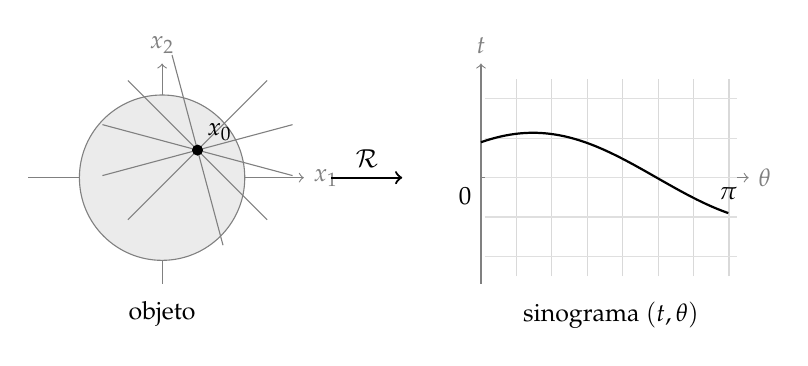
\begin{tikzpicture}[font=\small]
    \begin{scope}
        \draw[->, thin, gray] (-1.7,0) -- (1.8,0) node[right] {$x_1$};
        \draw[->, thin, gray] (0,-1.35) -- (0,1.45) node[above] {$x_2$};
        \draw[fill=black!8, draw=black!50] (0,0) circle (1.05);
        \coordinate (Xzero) at (0.45,0.35);
        \foreach \a in {15,45,75,105,135} {
            \draw[thin, gray] (Xzero) ++(\a+90:1.25) -- ++(\a-90:2.5);
        }
        \fill (Xzero) circle (2pt) node[above right] {$x_0$};
        \node[below] at (0,-1.45) {objeto};
    \end{scope}

    \draw[->, thick] (2.15,0) -- (3.05,0) node[midway, above] {$\mathcal R$};

    \begin{scope}[xshift=4.05cm]
        \draw[->, thin, gray] (0,0) -- (3.4,0) node[right] {$\theta$};
        \draw[->, thin, gray] (0,-1.35) -- (0,1.45) node[above] {$t$};
        \foreach \x in {0.45,0.9,...,3.15} {
            \draw[thin, gray!30] (\x,-1.25) -- (\x,1.25);
        }
        \foreach \y in {-1.0,-0.5,0,0.5,1.0} {
            \draw[thin, gray!25] (0.05,\y) -- (3.25,\y);
        }
        \draw[thick, black, domain=0:3.1416, samples=80, variable=\u]
            plot ({\u}, {0.45*cos(\u r)+0.35*sin(\u r)});
        \node[below left] at (0,0) {$0$};
        \node[below] at (3.14,0) {$\pi$};
        \node[align=center, below] at (1.65,-1.45) {sinograma $(t,\theta)$};
    \end{scope}
\end{tikzpicture}
\shorthandon{<>}
}
\caption{Formación esquemática del sinograma a partir de proyecciones paralelas. Elaboración propia.}
\label{fig:sinograma-diagrama}
\end{figure}

La linealidad se sigue directamente de la linealidad de la integral: para $f_1,f_2\in\mathcal S(\mathbb R^2)$ y escalares $a,b$,
\[
\mathcal R(af_1+bf_2)=a\mathcal Rf_1+b\mathcal Rf_2.
\]

Para identificar la retroproyección como adjunto formal, sea $D=\mathbb R\times(0,\pi)$. Para $u,v\in L^2(D)$ definimos el producto interno del espacio de datos por
\[
\langle u,v\rangle_{\mathrm{datos}}
=
\int_0^\pi\int_{\mathbb R}
u(t,\theta)\overline{v(t,\theta)}\,dt\,d\theta.
\]
Para $p\in L^1(\mathbb R^2)$ y $q\in L^\infty(\mathbb R^2)$ usamos la pareja de dualidad del espacio de imagen
\[
\langle p,q\rangle_{\mathrm{imagen}}
=
\int_{\mathbb R^2}p(x)\overline{q(x)}\,dx.
\]

Tomamos ahora $g\in C_c^\infty(D)$. Entonces $\mathcal Rf,g\in L^2(D)$ y $f\in L^1(\mathbb R^2)$. Definimos la retroproyección de $g$ por
\[
(\mathcal R^*g)(x)
=
\int_0^\pi
g(x\cdot\omega(\theta),\theta)\,d\theta.
\]
Además, $\mathcal R^*g\in L^\infty(\mathbb R^2)$, pues
\[
\|\mathcal R^*g\|_{L^\infty}
\leq
\pi\|g\|_{L^\infty}.
\]
Por consiguiente, en las parejas anteriores se toman concretamente $u=\mathcal Rf$, $v=g$, $p=f$ y $q=\mathcal R^*g$. Usando el cambio de variables
\[
x=t\omega(\theta)+s\omega^\perp(\theta),
\qquad dx=dt\,ds,
\]
para cada $\theta$, se obtiene
\[
\begin{aligned}
\langle\mathcal Rf,g\rangle_{\mathrm{datos}}
&=
\int_0^\pi\int_{\mathbb R}
(\mathcal Rf)(t,\theta)
\overline{g(t,\theta)}\,dt\,d\theta \\
&=
\int_{\mathbb R^2}
f(x)
\overline{
\left(
\int_0^\pi
g(x\cdot\omega(\theta),\theta)\,d\theta
\right)}\,dx \\
&=
\langle f,\mathcal R^*g\rangle_{\mathrm{imagen}}.
\end{aligned}
\]
Por tanto, la retroproyección $\mathcal R^*$ definida arriba es el adjunto formal de $\mathcal R$ con respecto a las medidas $dt\,d\theta$ y $dx$. La misma fórmula se empleará siempre que la integral angular esté bien definida. No se está afirmando aquí que ya se haya construido un operador acotado entre espacios $L^2$ completos. Para resultados de dualidad y retroproyección en un marco funcional más amplio puede consultarse Natterer \cite[Sec.~II.1, Thm.~1.3, pp.~13--15]{natterer2001}. Kuchment también desarrolla la retroproyección, aunque usa la notación $\mathcal R^\#$ y convenciones con integración angular diferentes \cite[Sec.~5.6, pp.~34--36]{kuchment2014}.

\section{Teorema de corte de Fourier}

El teorema de corte de Fourier conecta la transformada de Radon con la transformada de Fourier bidimensional. Con las convenciones del capítulo anterior, el resultado toma una forma directa.

\begin{theorem}[Teorema de corte de Fourier]
Sea $f\in\mathcal S(\mathbb R^2)$. Entonces, para todo $\theta\in[0,\pi)$ y $\sigma\in\mathbb R$,
\[
\mathcal F_t(\mathcal Rf)(\sigma,\theta)
=
\widehat f(\sigma\omega(\theta)).
\]
\end{theorem}

\begin{proof}
Usando la definición de $\mathcal Rf$ y el cambio de variables $x=t\omega(\theta)+s\omega^\perp(\theta)$, se tiene
\[
\begin{aligned}
\mathcal F_t(\mathcal Rf)(\sigma,\theta)
&=
\int_{\mathbb R}
\left(
\int_{\mathbb R}
f(t\omega(\theta)+s\omega^\perp(\theta))\,ds
\right)
e^{-2\pi i t\sigma}\,dt \\
&=
\int_{\mathbb R^2}
f(x)e^{-2\pi i\sigma x\cdot\omega(\theta)}\,dx \\
&=
\widehat f(\sigma\omega(\theta)).
\end{aligned}
\]
\end{proof}

Este resultado muestra que la transformada de Fourier unidimensional de una proyección proporciona los valores de $\widehat f$ sobre la recta radial
\[
\{\sigma\omega(\theta):\sigma\in\mathbb R\}
\]
en el dominio de frecuencias. Al variar $\theta\in[0,\pi)$, estas rectas cubren todo $\mathbb R^2$, aunque la parametrización es degenerada en el origen. El teorema de corte se encuentra, con posibles diferencias de normalización, en Helgason \cite{helgason1999}, Kuchment \cite[Sec.~5.5.4, Thm.~5.10, pp.~32--33]{kuchment2014} y Natterer \cite[Sec.~II.1, Thm.~1.1, p.~11]{natterer2001}; Kak y Slaney lo presentan en el contexto de proyecciones paralelas \cite[Sec.~3.2]{kak_slaney1988}.

\section{Fórmula de inversión}

Sea $f\in\mathcal S(\mathbb R^2)$. Partimos de la fórmula de inversión de Fourier en dos variables:
\[
f(x)=
\int_{\mathbb R^2}
\widehat f(\xi)e^{2\pi i x\cdot\xi}\,d\xi.
\]
Para reescribir esta integral en coordenadas adaptadas a la transformada de Radon, usamos el cambio con radio firmado
\[
\Phi(\sigma,\theta)=\sigma\omega(\theta),
\qquad
\sigma\in\mathbb R,
\quad
\theta\in[0,\pi).
\]
Para cada $\xi\neq0$ existe una única pareja
$(\sigma,\theta)\in(\mathbb R\setminus\{0\})\times[0,\pi)$
tal que $\xi=\sigma\omega(\theta)$. El origen es el único punto
degenerado de la parametrización y no afecta la integral.

Las derivadas del cambio son
\[
\partial_\sigma\Phi=\omega(\theta),
\qquad
\partial_\theta\Phi=\sigma\omega^\perp(\theta).
\]
Por tanto,
\[
\left|
\det\left(
\partial_\sigma\Phi,
\partial_\theta\Phi
\right)
\right|
=
|\sigma|.
\]
Así,
\[
d\xi=|\sigma|\,d\sigma\,d\theta.
\]

Sustituyendo en la inversión de Fourier y usando el teorema de corte,
\[
\begin{aligned}
f(x)
&=
\int_0^\pi\int_{\mathbb R}
\widehat f(\sigma\omega(\theta))
e^{2\pi i\sigma x\cdot\omega(\theta)}
|\sigma|\,d\sigma\,d\theta \\
&=
\int_0^\pi\int_{\mathbb R}
\mathcal F_t(\mathcal Rf)(\sigma,\theta)
|\sigma|
e^{2\pi i\sigma x\cdot\omega(\theta)}
\,d\sigma\,d\theta.
\end{aligned}
\]
Esta es la fórmula de inversión que se usará en la tesis. Con la convención de Fourier fijada y con integración angular en $[0,\pi)$, no aparece un factor adicional $1/2$ ni $1/\pi$ en esta expresión. Otras fuentes pueden usar frecuencia angular o integración sobre todas las direcciones, lo que modifica las constantes. La inversión de la transformada de Radon se desarrolla en Kuchment \cite[Sec.~5.7, pp.~36--39]{kuchment2014} y en Natterer \cite[Sec.~II.2, Thm.~2.1, pp.~18--20]{natterer2001}, con convenciones que deben convertirse antes de comparar factores.

\section{Retroproyección filtrada}

La fórmula de inversión anterior puede escribirse como un procedimiento operativo. Para cada ángulo $\theta$, se filtra la proyección $t\mapsto(\mathcal Rf)(t,\theta)$ en la variable del detector y luego se aplica la retroproyección.\\

El símbolo del filtro rampa es
\[
\tau_{\mathrm{rampa}}(\sigma)=|\sigma|.
\]
Con la notación de multiplicadores del capítulo anterior,
\[
T_{\tau_{\mathrm{rampa}}}h
=
\mathcal F_t^{-1}
\left[
|\sigma|\,\mathcal F_t h
\right].
\]
Para $f\in\mathcal S(\mathbb R^2)$, las proyecciones tienen regularidad suficiente para aplicar este multiplicador en la variable $t$.
Aplicado a cada proyección, esto produce el sinograma filtrado
\[
g_{\mathrm{filt}}(t,\theta)
=
\mathcal F_t^{-1}
\left[
|\sigma|\,\mathcal F_t(\mathcal Rf)(\sigma,\theta)
\right](t).
\]
La fórmula de inversión se convierte entonces en
\[
f
=
\mathcal R^*g_{\mathrm{filt}}
=
\mathcal R^*
\mathcal F_t^{-1}
\left[
|\sigma|\,\mathcal F_t(\mathcal Rf)
\right].
\]
Esta es la forma canónica de la retroproyección filtrada en esta tesis.
Equivalente y abreviadamente,
\[
f=\mathcal R^*T_{\tau_{\mathrm{rampa}}}\mathcal Rf,
\qquad
\tau_{\mathrm{rampa}}(\sigma)=|\sigma|.
\]

El factor $|\sigma|$ incorpora el jacobiano radial del cambio de variables, pero su crecimiento sin cota amplifica componentes de alta frecuencia. Esta observación conecta con la discusión de multiplicadores no acotados del capítulo anterior y motiva el estudio posterior de filtros modificados con símbolos $\tau(\sigma)$.

Escribiendo $g=\mathcal Rf$, la Figura~\ref{fig:fbp-flujo} presenta el procedimiento como una cadena de operaciones. Para un símbolo general $\tau$, la salida se denota $f_\tau$; para la rampa canónica $\tau(\sigma)=|\sigma|$, en el modelo continuo ideal se recupera $f$. En el capítulo computacional, la multiplicación por el símbolo se representará mediante el vector $M_\tau$, o la matriz diagonal asociada, aplicado a cada proyección en frecuencia.

\begin{figure}[htbp]
\centering
\resizebox{0.92\textwidth}{!}{\shorthandoff{<>}
\begin{tikzpicture}[node distance=1.35cm, font=\small]
    \tikzstyle{block}=[draw=black, fill=gray!10, rounded corners=2pt, minimum width=2.25cm, minimum height=0.78cm, align=center]
    \tikzstyle{data}=[align=center, minimum width=2.1cm]
    \node[data] (sino) {sinograma\\$g=\mathcal Rf$};
    \node[block, right=of sino] (fft) {Fourier en $t$\\$\mathcal F_t$};
    \node[data, right=of fft] (ghat) {$\widehat g(\sigma,\theta)$};
    \node[block, below=of ghat] (mult) {multiplicación por $\tau(\sigma)$\\(discreto: $M_\tau$)};
    \node[data, left=of mult] (gfhat) {$\widehat g_{\mathrm{filt}}$};
    \node[block, left=of gfhat] (ifft) {Fourier inversa\\$\mathcal F_t^{-1}$};
    \node[data, left=of ifft] (gf) {$g_{\mathrm{filt}}$};
    \node[block, below=of gf] (bp) {retroproyección\\$\mathcal R^*$};
    \node[data, right=of bp] (rec) {reconstrucción\\$f_\tau$};

    \draw[->, thick] (sino) -- (fft);
    \draw[->, thick] (fft) -- (ghat);
    \draw[->, thick] (ghat) -- (mult);
    \draw[->, thick] (mult) -- (gfhat);
    \draw[->, thick] (gfhat) -- (ifft);
    \draw[->, thick] (ifft) -- (gf);
    \draw[->, thick] (gf) -- (bp);
    \draw[->, thick] (bp) -- (rec);

    \node[align=center, below=0.45cm of mult]
    {rampa canónica continua: $\tau(\sigma)=|\sigma|$};
\end{tikzpicture}
\shorthandon{<>}
}
\caption{Flujo de la retroproyección filtrada en geometría paralela. Elaboración propia.}
\label{fig:fbp-flujo}
\end{figure}

La retroproyección filtrada es el algoritmo analítico clásico para datos de proyección paralela. Una presentación computacional se encuentra en Natterer \cite[Sec.~V.1, p.~102 y ss.]{natterer2001}; Kak y Slaney discuten la reconstrucción desde proyecciones paralelas en \cite[Sec.~3.3]{kak_slaney1988}. En esta tesis, la rampa se mantendrá como referencia teórica y computacional, mientras que las comparaciones numéricas posteriores reemplazarán $|\sigma|$ por otros símbolos $\tau(\sigma)$.


\chapter{Implementación numérica y análisis de la retroproyección filtrada}
\chaptermark{Implementación numérica y análisis de FBP}

En el capítulo anterior se estableció la fórmula continua de inversión por retroproyección filtrada y se fijó la convención
\[
f=\mathcal R^*\mathcal F_t^{-1}\bigl[|\sigma|\,\mathcal F_t(\mathcal Rf)\bigr].
\]
El objetivo de este capítulo es trasladar esa formulación a una implementación discreta reproducible, manteniendo la rampa canónica $\tau_{\mathrm{rampa}}(\sigma)=|\sigma|$ y evitando factores empíricos o normalizaciones ajustadas al fantoma.

El análisis se organiza alrededor de tres elementos: la discretización del modelo tomográfico, la aplicación de multiplicadores discretos en la variable del detector y la comparación de la rampa con seis filtros exploratorios. Los experimentos se realizan con un fantoma geométrico propio, una grilla espacial de tamaño $N=256$ y $M=90$ ángulos equiespaciados en $[0,\pi)$.

La discusión cuantitativa se apoya en métricas calculadas sobre el disco de soporte del fantoma. Los resultados no buscan identificar filtros óptimos, sino documentar cómo distintas elecciones del símbolo modifican el compromiso entre resolución y estabilidad frente al ruido bajo una configuración numérica fija.

\section{Discretización del modelo tomográfico}

La implementación numérica parte del modelo continuo descrito en los capítulos anteriores, pero reemplaza las funciones por arreglos finitos y las integrales por operaciones discretas. En esta sección se fijan las grillas espaciales, angulares y de detector usadas en todos los experimentos del capítulo.

\subsection*{Discretización del dominio espacial}

Se considera una malla cartesiana uniforme semiabierta en $[-1,1)^2$ de tamaño $N\times N$, con $N=256$. Con paso espacial $h=2/N$, los nodos se escriben como
\[
x_i=\left(i-\frac{N}{2}\right)h,\qquad
y_j=\left(j-\frac{N}{2}\right)h,
\qquad i,j=0,\ldots,N-1.
\]
Así, el índice $N/2=128$ representa exactamente el origen. Esta elección coincide con la convención de \texttt{scikit-image} 0.26.0, que sitúa el eje de rotación de \texttt{radon} en el píxel de índices \texttt{(N//2,N//2)} \cite{scikitimage_radon026}.
El fantoma utilizado es geométrico, asimétrico y está contenido en el disco
\[
x^2+y^2\le R^2,
\qquad R=0.9.
\]
No se usa el fantoma de Shepp--Logan como caso principal, porque se busca un objeto sintético simple con inclusiones de distintas intensidades y posiciones no simétricas.

\subsection*{Grilla angular y detector}

Los ángulos se toman uniformemente en $[0,\pi)$ mediante
\[
\theta_k=k\Delta\theta,
\qquad k=0,\ldots,M-1,
\]
con
\[
M=90,
\qquad \Delta\theta=2^\circ=\frac{\pi}{90}.
\]
Para cada ángulo se genera una proyección discreta, y el conjunto de proyecciones forma un sinograma
\[
g\in\mathbb R^{N_t\times M},
\qquad N_t=256.
\]
La variable del detector se discretiza como
\[
t_\ell=(\ell-N_t/2)\Delta t,
\qquad \ell=0,\ldots,N_t-1,
\]
donde $\Delta t=h=2/N$. El índice $N_t/2=128$ corresponde exactamente a $t=0$ y coincide con el eje del sinograma, que la implementación ubica en \texttt{N\_t//2} \cite{scikitimage_radon026}.

\subsection*{Generación del sinograma}

El sinograma se genera con la rutina \texttt{radon} de \texttt{scikit-image} \cite{vanderwalt2014scikitimage}, usando la opción \texttt{circle=True}. En la versión 0.26.0, esta opción supone que la imagen es nula fuera del círculo inscrito en la malla y hace que el ancho de cada proyección sea igual a la menor dimensión de la imagen \cite{scikitimage_radon026}; por ello se conserva $N_t=N=256$. No describe una geometría de adquisición circular: la adquisición sigue correspondiendo a una geometría de haz paralelo.\\

La definición geométrica continua no se modifica: la recta asociada a $(t,\theta)$ sigue dada por $x\cdot\omega(\theta)=t$, con $\omega(\theta)=(\cos\theta,\sin\theta)$. La implementación debe, sin embargo, distinguir esta convención matemática de la orientación vertical de las matrices digitales, cuyas filas crecen en sentido opuesto al eje cartesiano usual. Esta diferencia se corrige al retroproyectar, sin cambiar la definición de la transformada de Radon.\\

La Figura~\ref{fig:chapter3-phantom-sinogram} muestra el fantoma y el sinograma generado con estos parámetros.

\begin{figure}[htbp]
    \centering
    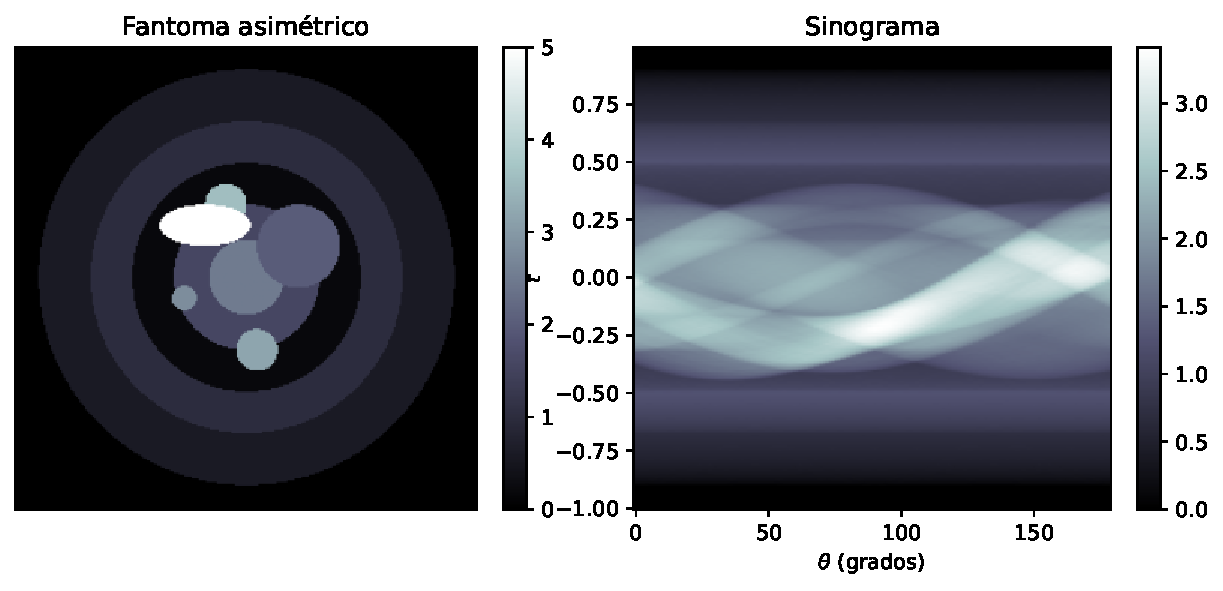
\includegraphics[width=0.92\textwidth]{Figures/Chapter3/phantom_and_sinogram.pdf}
    \caption{Fantoma geométrico utilizado en los experimentos y sinograma generado con $M=90$ ángulos de haz paralelo. El fantoma está contenido en el disco de radio $R=0.9$, y el sinograma constituye el dato de entrada para las reconstrucciones posteriores.}
    \label{fig:chapter3-phantom-sinogram}
\end{figure}

Esta discretización es suficiente para estudiar el comportamiento relativo de los filtros considerados. Existen formulaciones formales de transformadas de Radon discretas, como la de Beylkin \cite{beylkin1987}, pero la implementación de esta tesis corresponde a un modelo muestreado basado en sinogramas generados numéricamente y no a una implementación exacta de dicha transformada discreta. Los errores introducidos por interpolación, muestreo espacial y muestreo angular forman parte del modelo numérico evaluado y no se corrigen mediante ajustes posteriores de amplitud \cite{kak_slaney1988,natterer2001}.

\section{Algoritmo discreto de retroproyección filtrada}

La retroproyección filtrada discreta implementa la fórmula continua de FBP mediante operaciones finitas en la variable del detector y una cuadratura angular. En esta sección se separan la retroproyección sin filtrar, el filtrado por columnas y la reconstrucción final.

\subsection*{Retroproyección discreta}

El operador continuo de retroproyección está dado por
\[
\mathcal R^*g(x)=\int_0^\pi g(x\cdot\omega(\theta),\theta)\,d\theta,
\]
con $\omega(\theta)=(\cos\theta,\sin\theta)$. En la malla discreta se aproxima por
\[
(\mathcal R_d^*g)_{i,j}
=
\Delta\theta\sum_{k=0}^{M-1}
\mathcal I_t\bigl[g_{\cdot,k}\bigr]
\bigl(t(x_i,y_j,\theta_k)\bigr),
\]
donde $\mathcal I_t$ denota interpolación lineal en la variable del detector. La geometría matemática usa $t(x,y,\theta)=x\cdot\omega(\theta)$; en la implementación matricial se toma en cuenta la orientación vertical de las filas para evaluar correctamente las coordenadas cartesianas.

La retroproyección sin filtrar se obtiene aplicando directamente este operador al sinograma:
\[
f_{\mathrm{BP}}=\mathcal R_d^*g.
\]
Como se discutió en el capítulo anterior, $\mathcal R^*\mathcal R$ no es la identidad; por ello esta reconstrucción presenta difuminado y requiere filtrado previo.

\subsection*{Filtrado discreto por columnas}

El filtrado se aplica independientemente a cada columna angular $g_{\cdot,k}\in\mathbb R^{N_t}$. Para distinguir la transformada de Fourier continua de la transformada discreta usada en el código, se introducen los siguientes operadores:
\begin{itemize}
    \item $P:\mathbb R^{N_t}\to\mathbb R^{N_{\mathrm{fft}}}$, operador de zero-padding centrado.
    \item $C:\mathbb R^{N_{\mathrm{fft}}}\to\mathbb R^{N_t}$, operador de recorte al intervalo detector original.
    \item $F_{N_{\mathrm{fft}}}$, DFT de longitud $N_{\mathrm{fft}}$.
    \item $M_\tau[m]=\tau(\sigma_m)$, vector multiplicador evaluado en la grilla de frecuencias $\sigma_m$ generada con \texttt{fftfreq}.
\end{itemize}

Para cada columna angular se calcula
\[
g^\tau_{\cdot,k}
=
C F_{N_{\mathrm{fft}}}^{-1}
\operatorname{diag}(M_\tau)
F_{N_{\mathrm{fft}}}
P g_{\cdot,k}.
\]
En los experimentos se usa
\[
N_t=256,
\qquad
N_{\mathrm{fft}}=1024.
\]
La longitud $N_{\mathrm{fft}}$ es auxiliar: no añade datos ni resolución espacial. Su función es reducir los efectos de tratar directamente cada proyección finita como si fuera periódica, es decir, mitigar artefactos asociados a la convolución circular de la DFT.

\subsection*{Reconstrucción filtrada}

Luego de filtrar todas las columnas, la reconstrucción se define como
\[
f_\tau=\mathcal R_d^*g^\tau.
\]
Para la rampa canónica,
\[
\tau_{\mathrm{rampa}}(\sigma)=|\sigma|,
\]
esta expresión es la contraparte discreta de
\[
f=\mathcal R^*\mathcal F_t^{-1}\bigl[|\sigma|\,\mathcal F_t(\mathcal Rf)\bigr].
\]
No se introducen factores $1/2$, $1/\pi$, correcciones empíricas ni reescalamientos de las reconstrucciones.

La Figura~\ref{fig:chapter3-bp-vs-fbp} compara la retroproyección sin filtrar con la reconstrucción FBP usando la rampa.

\begin{figure}[htbp]
    \centering
    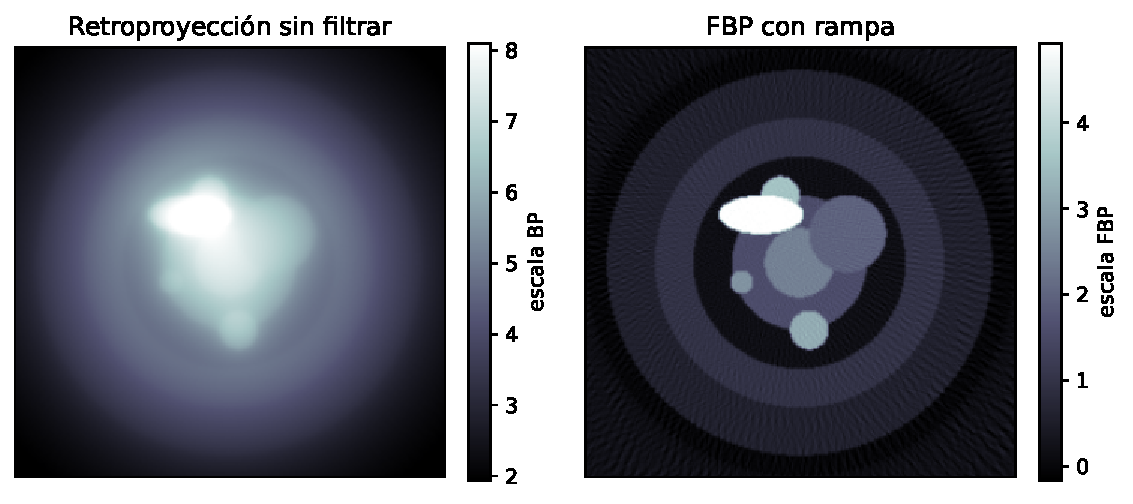
\includegraphics[width=0.86\textwidth]{Figures/Chapter3/bp_vs_fbp.pdf}
    \caption{Comparación entre la retroproyección sin filtrar y la retroproyección filtrada con la rampa. La retroproyección directa produce una imagen difuminada, mientras que el filtrado previo compensa parcialmente el suavizado asociado a $\mathcal R^*\mathcal R$.}
    \label{fig:chapter3-bp-vs-fbp}
\end{figure}

\section{Símbolos discretos y filtros A--F}

El algoritmo anterior queda determinado por el símbolo $\tau$ usado para construir el multiplicador discreto $M_\tau$. En esta sección se describen los siete símbolos evaluados: la rampa como referencia y seis filtros exploratorios, denotados A--F.

\subsection*{Rampa de referencia}

El símbolo de referencia es la rampa canónica
\[
\tau_{\mathrm{rampa}}(\sigma)=|\sigma|.
\]
Esta elección corresponde directamente a la fórmula continua de FBP fijada en el Capítulo 2. En la implementación discreta no se introduce ningún factor adicional en este símbolo.

\subsection*{Filtros exploratorios A, B y C}

El filtro A modifica la rampa mediante una perturbación oscilatoria dependiente de la frecuencia:
\[
\tau_A(\sigma)
=
|\sigma|\left(1+\frac{\sin|\sigma|}{1+|\sigma|}\right).
\]
El filtro B tiene respuesta no nula en frecuencia cero:
\[
\tau_B(\sigma)=\sqrt{0.3^2+|\sigma|^2}.
\]
En particular, $\tau_B(0)=0.3$. En cambio, la rampa y los filtros A, C, D, E y F se anulan en frecuencia cero.\\

El filtro C introduce un corte compacto relativo a la frecuencia máxima de la grilla discreta:
\[
\tau_C(\sigma)
=
|\sigma|\left(1-\frac{|\sigma|}{\sigma_c}\right)_+,
\qquad
\sigma_c=0.6\sigma_{\max}.
\]
Aquí $(a)_+=\max\{a,0\}$.

\subsection*{Filtros D, E y F}

Los filtros D, E y F crecen como la rampa hasta $|\sigma|=20$ y luego modifican el tratamiento de frecuencias mayores. El filtro D es triangular:
\[
\tau_D(\sigma)=
\begin{cases}
|\sigma|, & |\sigma|\le 20,\\
40-|\sigma|, & 20<|\sigma|\le 40,\\
0, & |\sigma|>40.
\end{cases}
\]
El filtro E usa decaimiento exponencial moderado:
\[
\tau_E(\sigma)=
\begin{cases}
|\sigma|, & |\sigma|\le 20,\\
20\exp[-0.08(|\sigma|-20)], & |\sigma|>20.
\end{cases}
\]
El filtro F usa decaimiento exponencial más rápido:
\[
\tau_F(\sigma)=
\begin{cases}
|\sigma|, & |\sigma|\le 20,\\
20\exp[-0.50(|\sigma|-20)], & |\sigma|>20.
\end{cases}
\]

Estos seis filtros no se presentan como filtros óptimos. Su propósito es explorar, bajo una misma configuración numérica, cómo distintas respuestas espectrales alteran la reconstrucción y su sensibilidad al ruido. Esta pregunta se relaciona con el análisis de error y el diseño de funciones filtro en FBP \cite{beckmann_iske2017,beckmann_nickel2025}, pero los símbolos A--F usados aquí no se derivan de esos trabajos ni reproducen sus filtros optimizados.

La Figura~\ref{fig:chapter3-symbols} muestra la rampa y los filtros A--F sobre la grilla de frecuencias usada por la DFT.

\begin{figure}[htbp]
    \centering
    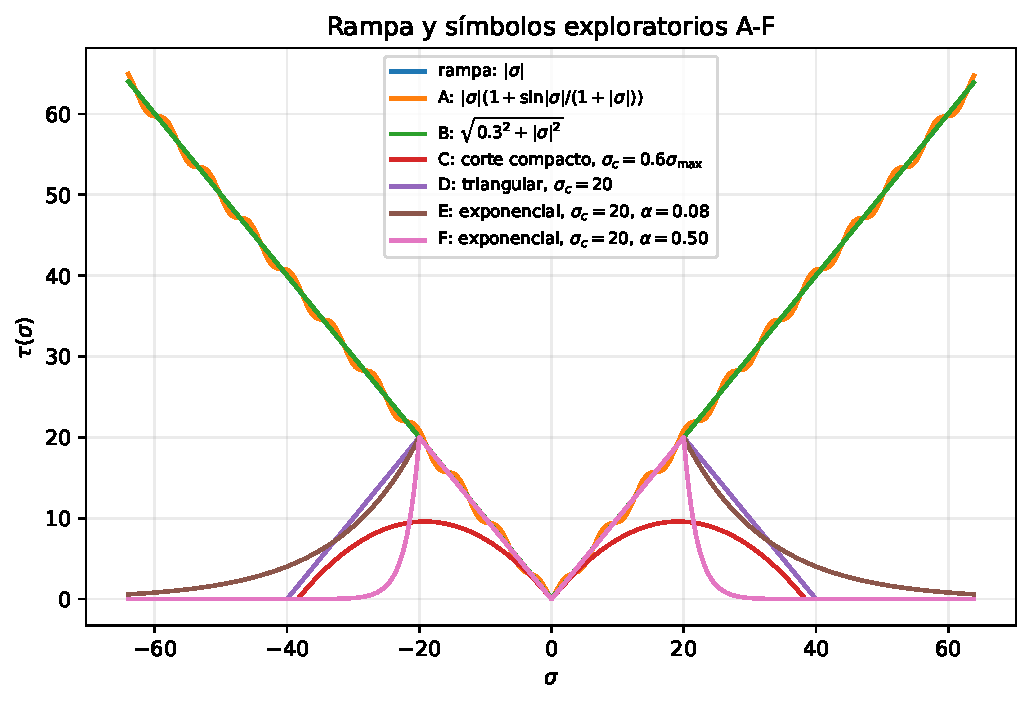
\includegraphics[width=0.86\textwidth]{Figures/Chapter3/symbols_ramp_A_F.pdf}
    \caption{Símbolos discretos evaluados sobre la grilla de frecuencias de longitud $N_{\mathrm{fft}}=1024$. La rampa se usa como referencia; los símbolos A--F son filtros exploratorios para estudiar el efecto de distintas modificaciones espectrales.}
    \label{fig:chapter3-symbols}
\end{figure}

\section{Diseño experimental y reproducibilidad}

Los experimentos del capítulo se generan de forma reproducible a partir del código incorporado en el repositorio. Esta sección resume los parámetros, el modelo de ruido, las métricas y las verificaciones automáticas usadas para producir las figuras y tablas.

\subsection*{Parámetros canónicos}

La configuración numérica es fija en todos los experimentos:
\[
N=256,
\qquad
R=0.9,
\qquad
N_t=256,
\qquad
N_{\mathrm{fft}}=1024,
\]
\[
M=90,
\qquad
\Delta\theta=2^\circ,
\qquad
\texttt{circle=True}.
\]
La opción \texttt{circle=True} impone la hipótesis de soporte en el círculo inscrito y mantiene $N_t=256$ muestras de detector; no modifica la geometría de adquisición de haz paralelo. La longitud $N_{\mathrm{fft}}=1024$ se usa solo como longitud auxiliar para el filtrado por FFT con zero-padding centrado.\\

El código de reproducción se ejecuta desde la raíz del repositorio mediante
\[
\texttt{python code/generate\_chapter3.py}.
\]
Las versiones de NumPy, SciPy, scikit-image y Matplotlib están fijadas en el archivo de requisitos del código. Los detalles de cada corrida se registran en los metadatos de resultados, y la auditoría de normalización queda guardada junto con esos resultados.

\subsection*{Ruido}

Para evaluar estabilidad se añade ruido gaussiano aditivo al sinograma:
\[
g_{\mathrm{ruido}}=g+\eta,
\qquad
\eta_{\ell,k}\sim\mathcal N(0,\sigma_{\mathrm{noise}}^2),
\]
con
\[
\sigma_{\mathrm{noise}}=0.05\max |g|.
\]
La semilla aleatoria es $42$, y la misma realización ruidosa se usa para todos los filtros. Por tanto, las diferencias observadas bajo ruido se deben al filtrado y no a cambios en la muestra aleatoria.

\subsection*{Métricas}

Las métricas se calculan únicamente sobre los índices correspondientes al disco de soporte del fantoma:
\[
\mathcal I_R=\{(i,j):x_i^2+y_j^2\le R^2\}.
\]
Si $u$ es el fantoma y $v$ una reconstrucción, se usa
\[
\mathrm{RMSE}(u,v)
=
\left(
\frac{1}{\#\mathcal I_R}
\sum_{(i,j)\in\mathcal I_R}
(u_{i,j}-v_{i,j})^2
\right)^{1/2},
\]
y el error relativo en norma discreta $\ell^2$,
\[
\mathrm{Err}_{\ell^2}(u,v)
=
\frac{
\left(\sum_{(i,j)\in\mathcal I_R}(u_{i,j}-v_{i,j})^2\right)^{1/2}
}{
\left(\sum_{(i,j)\in\mathcal I_R}u_{i,j}^2\right)^{1/2}
}.
\]
La tabla de resultados también reporta la razón de medias entre reconstrucción y fantoma sobre $\mathcal I_R$. Esta cantidad se conserva solo como diagnóstico de amplitud; no es una métrica principal ni se utiliza como factor de escala.

\subsection*{Verificaciones automáticas}

La generación comprueba dimensiones de imagen, sinograma y multiplicadores; ausencia de valores no finitos; paridad de los símbolos; valores en frecuencia cero; aplicación independiente por columnas; orientación espacial; y reproducibilidad del hash de métricas al ejecutar dos veces con la misma semilla. No se normalizan las reconstrucciones contra el fantoma ni se aplica corrección empírica de amplitud.

\section{Resultados y discusión}

Esta sección integra las reconstrucciones y métricas generadas con la configuración descrita. La interpretación se limita a los filtros evaluados, al fantoma usado y a la realización de ruido considerada.

\subsection*{Reconstrucciones sin ruido}

La Figura~\ref{fig:chapter3-recon-noiseless} muestra las reconstrucciones obtenidas a partir del sinograma sin ruido. Visualmente, la rampa recupera la estructura principal del fantoma y obtiene el menor error relativo, mientras que los filtros E y D producen resultados cercanos entre sí según las métricas de la Tabla~\ref{tab:chapter3-metrics}.

\begin{figure}[htbp]
    \centering
    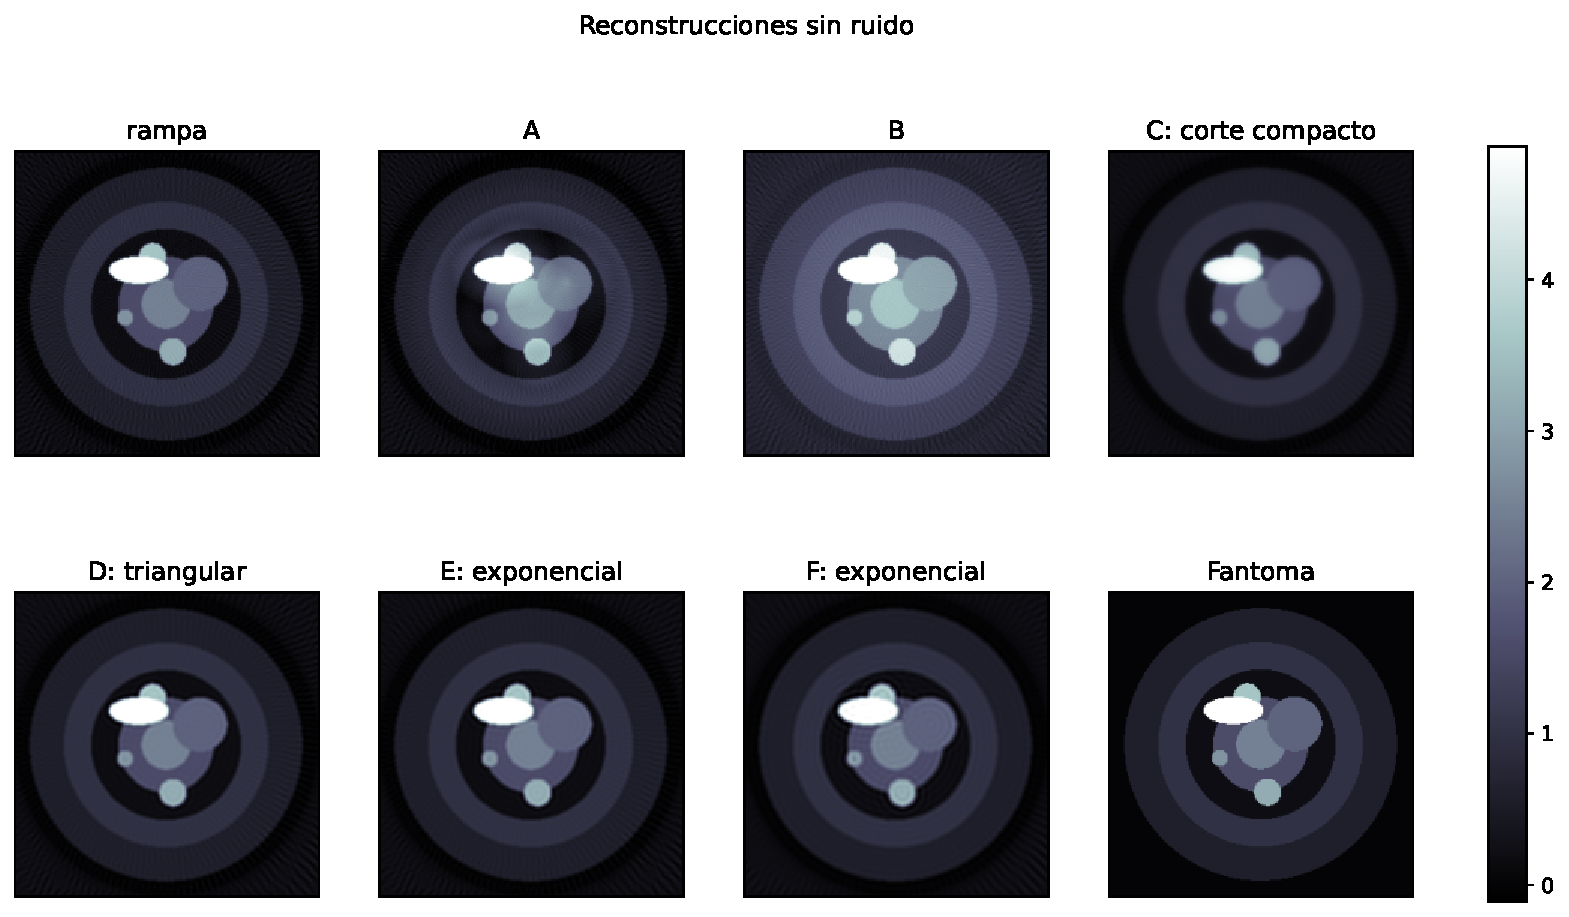
\includegraphics[width=0.96\textwidth]{Figures/Chapter3/reconstructions_noiseless.pdf}
    \caption{Reconstrucciones obtenidas sin ruido para la rampa y los filtros A--F. El último panel muestra el fantoma de referencia bajo la misma escala de color usada para las reconstrucciones, lo que permite comparar amplitud y estructura visual.}
    \label{fig:chapter3-recon-noiseless}
\end{figure}

En términos de error relativo, el menor valor sin ruido corresponde a la rampa, con $0.097892$. Le siguen E, con $0.112767$, y D, con $0.113110$; la diferencia entre estos dos filtros es pequeña en esta configuración. F obtiene $0.127115$ y C alcanza $0.143042$, mientras que A y B presentan errores mayores, $0.253226$ y $0.687715$, respectivamente.

\subsection*{Reconstrucciones con ruido}

La Figura~\ref{fig:chapter3-recon-noisy} muestra las reconstrucciones obtenidas a partir del sinograma perturbado con ruido gaussiano. Bajo la realización de ruido considerada, los filtros que atenúan altas frecuencias reducen de forma marcada la amplificación del ruido respecto de la rampa.

\begin{figure}[htbp]
    \centering
    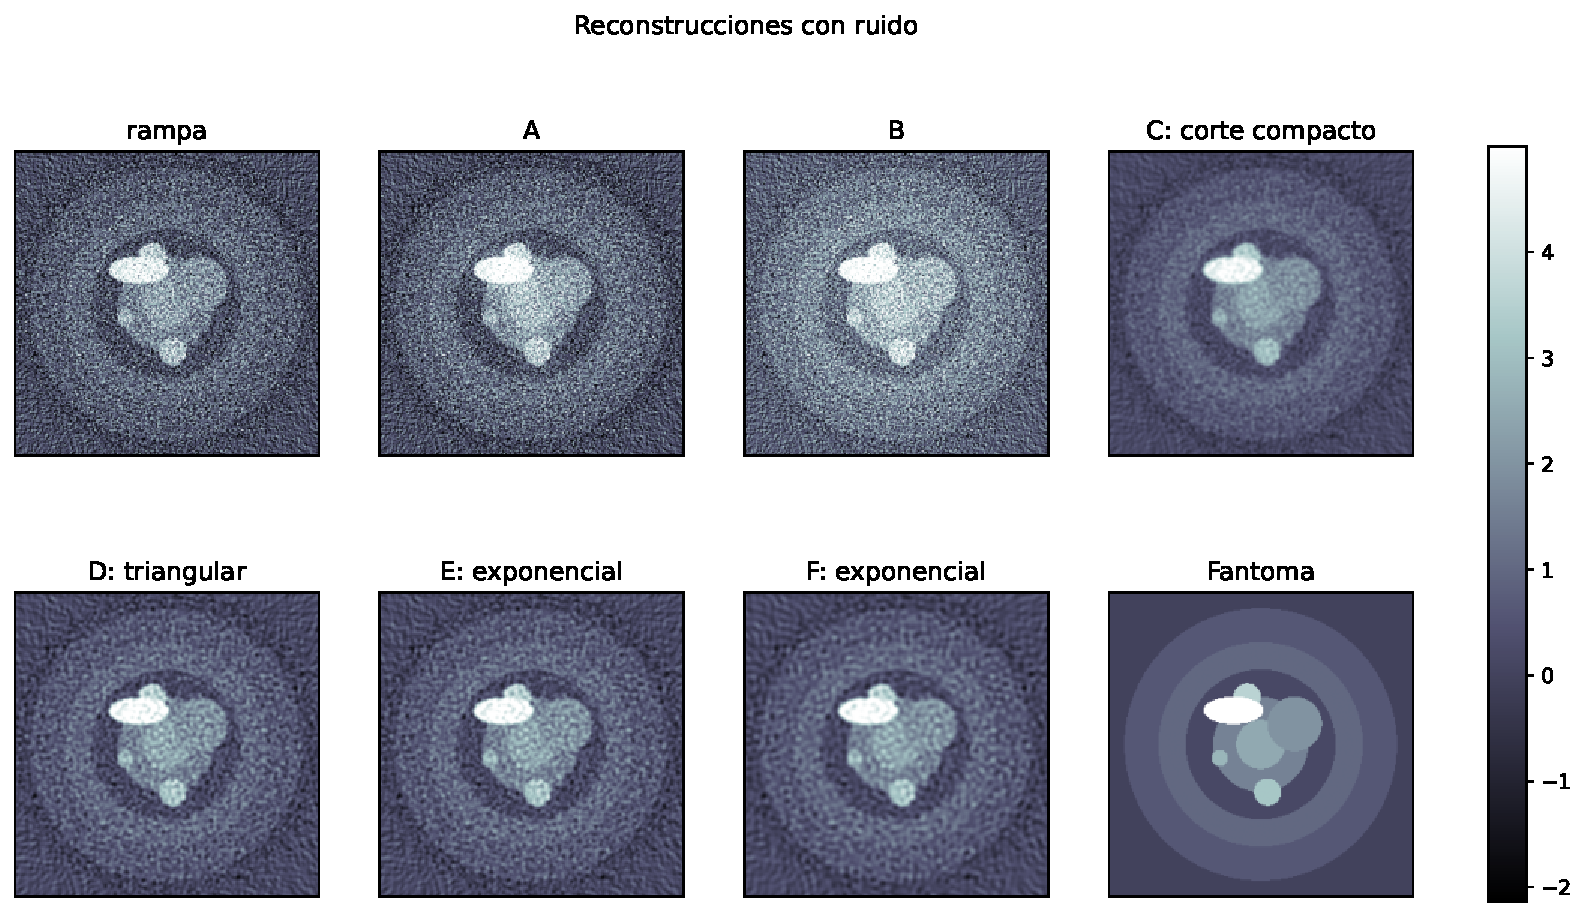
\includegraphics[width=0.96\textwidth]{Figures/Chapter3/reconstructions_noisy.pdf}
    \caption{Reconstrucciones obtenidas a partir de un único sinograma ruidoso, común a todos los filtros. Las diferencias visuales reflejan el compromiso entre preservación de detalle y atenuación de altas frecuencias bajo la realización de ruido considerada.}
    \label{fig:chapter3-recon-noisy}
\end{figure}

Entre los filtros evaluados, C obtiene el menor error relativo con ruido, $0.266386$, seguido por F con $0.318981$. Los filtros E y D quedan en un rango intermedio, con $0.383664$ y $0.390949$, respectivamente. La rampa y A presentan errores relativos mayores, $1.134227$ y $1.157932$, consistentes con una mayor amplificación de altas frecuencias. El filtro B alcanza $1.323399$; su comportamiento desfavorable es consistente con su respuesta no nula en frecuencia cero y su mayor peso de bajas frecuencias, aunque este experimento no constituye una demostración causal completa.

\subsection*{Métricas cuantitativas}

La Tabla~\ref{tab:chapter3-metrics} resume RMSE, error relativo y razón de medias. RMSE y error relativo son las métricas principales. La razón de medias se incluye únicamente como diagnóstico de amplitud y no se usa para reescalar ni para seleccionar filtros.

\begin{table}[htbp]
    \centering
    \caption{Métricas de reconstrucción calculadas sobre los índices $\mathcal I_R=\{(i,j):x_i^2+y_j^2\le R^2\}$. RMSE y error relativo en norma $\ell^2$ son las métricas principales; la razón de medias se reporta únicamente como diagnóstico de amplitud.}
    \label{tab:chapter3-metrics}
    \small
    \begin{tabular}{llrrr}
\toprule
Caso & Filtro & RMSE & Error relativo $\ell^2$ & Razón media \\
\midrule
sin ruido & rampa & 0.125294 & 0.097892 & 0.976683 \\
sin ruido & A & 0.324107 & 0.253226 & 1.181567 \\
sin ruido & B & 0.880214 & 0.687715 & 1.906510 \\
sin ruido & C: corte compacto & 0.183081 & 0.143042 & 0.963424 \\
sin ruido & D: triangular & 0.144770 & 0.113110 & 0.975620 \\
sin ruido & E: exponencial & 0.144332 & 0.112767 & 0.975596 \\
sin ruido & F: exponencial & 0.162695 & 0.127115 & 0.975090 \\
con ruido & rampa & 1.451709 & 1.134227 & 0.978050 \\
con ruido & A & 1.482050 & 1.157932 & 1.183776 \\
con ruido & B & 1.693833 & 1.323399 & 1.908387 \\
con ruido & C: corte compacto & 0.340951 & 0.266386 & 0.964867 \\
con ruido & D: triangular & 0.500380 & 0.390949 & 0.977034 \\
con ruido & E: exponencial & 0.491055 & 0.383664 & 0.977022 \\
con ruido & F: exponencial & 0.408268 & 0.318981 & 0.976554 \\
\bottomrule
\end{tabular}

\end{table}

Los resultados ilustran el compromiso entre resolución y estabilidad: sin ruido, las respuestas próximas a la rampa conservan mejor los detalles; con ruido, atenuar altas frecuencias reduce el error a costa de suavizado. El desempeño de C se limita a esta configuración y realización de ruido, sin implicar superioridad universal.


\chapter{Conclusiones}

Esta tesis presentó un estudio de la retroproyección filtrada en reconstrucción tomográfica bidimensional, combinando derivación matemática e implementación reproducible. En el modelo continuo se fijaron las convenciones de Fourier, la parametrización normal de las rectas y el intervalo angular $\theta\in[0,\pi)$. Con ellas, la transformada de Radon se relacionó con la transformada de Fourier bidimensional mediante el teorema de corte, y la fórmula de FBP se obtuvo por el cambio a coordenadas polares con radio firmado. Así se identificó el filtro rampa $\tau_{\mathrm{rampa}}(\sigma)=|\sigma|$ como el factor espectral asociado al jacobiano radial, sin factores adicionales de normalización.

La parte computacional trasladó esta formulación a un esquema discreto reproducible con un fantoma geométrico propio, sinogramas de haz paralelo bajo la hipótesis de soporte en el círculo inscrito, filtrado por columnas mediante FFT con relleno centrado de ceros y retroproyección discreta. La rampa se mantuvo como referencia teórica y numérica, mientras que los filtros A--F se usaron como modificaciones exploratorias del símbolo para observar cómo distintas respuestas espectrales afectan la reconstrucción.

Los experimentos muestran el compromiso esperado entre resolución y estabilidad. Sin ruido, los filtros D y E obtuvieron los menores errores relativos y quedaron prácticamente empatados; la rampa produjo un resultado cercano y conservó su papel de referencia. Con ruido, bajo la configuración y la realización aleatoria consideradas, el filtro C alcanzó el menor error relativo. Esta observación no implica superioridad universal del filtro C, sino una conclusión restringida al fantoma, al nivel de ruido, a la semilla y a los parámetros numéricos utilizados.

Las limitaciones del estudio son deliberadas: geometría paralela bidimensional, fantoma sintético, una sola realización de ruido y filtros exploratorios. No se usaron datos clínicos ni tridimensionales, no se ajustó empíricamente la amplitud de las reconstrucciones y no se intentó demostrar optimalidad. Estas restricciones permitieron mantener una conexión clara entre la fórmula continua de FBP, su implementación discreta y la interpretación de los resultados.

Como trabajo futuro, sería natural ampliar los experimentos a múltiples semillas aleatorias, otros niveles de ruido, otras familias de fantomas y criterios cuantitativos adicionales. También podría estudiarse el diseño sistemático de filtros bajo objetivos de error o estabilidad, así como configuraciones con datos incompletos o de ángulo limitado \cite{quinto1993,frikel_quinto2013}.


%%%%%%%%%%%%%%%%%%%%%%%%%%%%%%%%%%%%%%%%%%%%%%%%%%%%%%%%%%%%%
% REFERENCIAS
%%%%%%%%%%%%%%%%%%%%%%%%%%%%%%%%%%%%%%%%%%%%%%%%%%%%%%%%%%%%%

\selectlanguage{spanish}

\setlength{\emergencystretch}{3em}
\sloppy

% \nocite{*}
{%
\small
\setlength{\bibitemsep}{0pt}
\setlength{\bibparsep}{0pt}
\printbibliography[heading=bibintoc,title={Bibliografía}]
}

\selectlanguage{spanish}

\end{document}
